

%----------------------------------------------------------------------------------------
%	PACKAGES AND OTHER DOCUMENT CONFIGURATIONS 
%----------------------------------------------------------------------------------------

\documentclass[paper=a4, fontsize=11pt]{scrartcl} % A4 paper and 11pt font size

\usepackage[T1]{fontenc} % Use 8-bit encoding that has 256 glyphs
\usepackage{fourier} % Use the Adobe Utopia font for the document - comment this line to return to the LaTeX default
\usepackage[english]{babel} % English language/hyphenation
\usepackage{amsmath,amsfonts,amsthm} % Math packages

\usepackage{lipsum} % Used for inserting dummy 'Lorem ipsum' text into the template



\usepackage{sectsty} % Allows customizing section commands
\allsectionsfont{\centering \normalfont\scshape} % Make all sections centered, the default font and small caps

\usepackage{graphicx}

\usepackage{fancyhdr} % Custom headers and footers
\pagestyle{fancyplain} % Makes all pages in the document conform to the custom headers and footers
\fancyhead{} % No page header - if you want one, create it in the same way as the footers below
\fancyfoot[L]{} % Empty left footer
\fancyfoot[C]{} % Empty center footer
\fancyfoot[R]{\thepage} % Page numbering for right footer
\renewcommand{\headrulewidth}{0pt} % Remove header underlines
\renewcommand{\footrulewidth}{0pt} % Remove footer underlines
\setlength{\headheight}{13.6pt} % Customize the height of the header

\numberwithin{equation}{section} % Number equations within sections (i.e. 1.1, 1.2, 2.1, 2.2 instead of 1, 2, 3, 4)
\numberwithin{figure}{section} % Number figures within sections (i.e. 1.1, 1.2, 2.1, 2.2 instead of 1, 2, 3, 4)
\numberwithin{table}{section} % Number tables within sections (i.e. 1.1, 1.2, 2.1, 2.2 instead of 1, 2, 3, 4)

\setlength\parindent{0pt} % Removes all indentation from paragraphs - comment this line for an assignment with lots of text

%----------------------------------------------------------------------------------------
%	TITLE SECTION
%----------------------------------------------------------------------------------------

\newcommand{\horrule}[1]{\rule{\linewidth}{#1}} % Create horizontal rule command with 1 argument of height

\title{	
\normalfont \normalsize 
\textsc{University of the Witwatersrand, School of Electrical and Information Engineering} \\ [25pt] % Your university, school and/or department name(s)
\horrule{0.5pt} \\[0.4cm] % Thin top horizontal rule
\huge Software Engineering: ELEN4009 \\ Project 13  Fleet of Delivery and Pick-up Vehicle Management System Project Report \\ % The assignment title
\horrule{2pt} \\[0.5cm] % Thick bottom horizontal rule
}

\author{Front End \\ Sheena Philip (545819),\\ Kessigan Subramanium (573799),\\  Back end \\ Linda Khumalo (560895), \\  Phumzile Dlwathi(545290)}




\date{11 April 2016} % Today's date or a custom date


\begin{document}

\newpage

\maketitle % Print the title
\newpage

\tableofcontents

%\maketitle % Print the title

%----------------------------------------------------------------------------------------
%	PROBLEM 1
%----------------------------------------------------------------------------------------
\newpage
\section{INTRODUCTION}



\subsection{Problem Statement}

CourierJZ is a courier company that is based in the Gauteng region and has one depot in Johannesburg which is responsible for all its operations in the area. Courier JZ currently uses an inefficient, time consuming, tedious system which is not centralised or automated to manage their fleet of delivery and pick-up vehicles.  This means that parcels are not being delivered in the shortest time possible since calculations and allocation of resources in the company is performed manually, making the company less competitive. In addition since the system is not automated and centralised on the web, clients enquiring about the process and getting information and monitoring their parcel becomes tedious, giving the customer a bad experience which ultimately gives the company an unfavourable brand image. \\

The company is tasked with developing a complete back and front end system to replace the paper system currently in use. The system must be able to log packages for collections and allocate drivers to pick them up and return them to the depot for processing. The system will also then need to efficiently sort the packages for delivery, with the shortest delivery time being prioritised. \\

CourierJZ should pick up and deliver parcels from and to its' respective customers in the shortest time and in the most efficient and least troublesome/interfering way possible. A parcel should also be able to be tracked from it pick-up point to its delivery point, allowing the company to have better control over the system and allowing customers to be better informed about their parcel. \\

This system will provide a web interface that allows senders to request and pay for deliveries while also allowing receivers to track their packages. The system will also provide an online interface that allows the workers easy access to the company's information when they log on to the website. The internal processes will all be managed by the companies stakeholders that have their own dashboards that correspond to the role they play in the company.\\



\subsection{Problem Objectives}
\begin{itemize}
\item To design, implement and test a web-based management system for a fleet of delivery and pick-up vehicles
\item The website must serve as a platform to integrate the various activities of the personnel involved in the day to day running of the business
\item The website must automate previously time-consuming activities resulting in a  more efficient company.
\item The website must act as a repository  to store all the data associated with the business activities.
\item The website must serve as a more convenient and efficient way for a client to be informed about the services available and to track their parcel.
\end{itemize}

\subsection{Stakeholders}
The following are the stakeholders involved in the project:
\begin{itemize}
\item Four software developers
\item Driver
\item CEO
\item Clients
\item Operational officer
\item Fleet assignment manager
\item Vehicle maintenance manager
\item System administrator
\item Account officer
\end{itemize}

\subsection{PROJECT DELIVERABLES}


\begin{itemize}
\item Tracking of parcels
\item Tracking of vehicles
\item Design shortest distance route algorithm
\item Determine the vehicle certain packages go into
\item Allow a driver to choose a vehicle and a route
\item Determine date and time of package pickup
\item Determine date and time of delivery
\item Store payment information
\item Store client details
\item Package storage and package identification
\item Send automated email notifications to clients
\item Inventory management
\end{itemize}

\section{Design}

\subsection{Existing Solutions}
DHL is a globally known delivery company that delivers packages both locally and internationally. They have two options when delivering packages, the customer can either request online for DHL to go to the customer's location and pick up the package for delivery or the customer can go to one of DHL's many branches in order to drop off the package. The site offers the customer a choice of many delivery options and the estimated price for that option, these options have various prices depending on when the delivery is expected to be made \cite{DHL}.\\

Aramex is a similar delivery company to DHL and allows the customer to request an online pick up or a store-to-door option which lets customers drop off their packages at local retailers like pick n' pay. The websites of both these companies have homepages packed with information and the relevant links, the pages seem crowded at first but allow the customer to view all option before selecting one. These sites also show price, delivery estimations and allow senders or receivers to track their packages. The websites only gives information and views for what the customer would need and has no indication of the internal working of the company, e.g. how drivers see package details or how the packages are routed to their destinations. \cite{Aramex}
\\

Fastway is another global courier service. They offer many of the services that are offered by DHL. In addition the company offers a service called the Fastlabel automatic label printing. This is a system that allows a user to print the labels required to be stuck on to the packages at home. This reduces dispatch labour requirements which overall reduces the cost of the service. Fastway's website also allows companies to make their service an API on the company's respective websites which helps market the service and improves the user experience. Fastway's website is simple, non-crowded and has an effective use of pictures in order to explain certain concepts and navigate a client around \cite{Fastway}.
\\

Telogis is an award winning , fleet management software developing company. This company has developed one of the best softwares' for  fleet management. The system features that stood out were: the real time tracking for both customer and the fleet mananger, Progress against planned routes, fuel usage and an estimated cost that the company will incur for a certain delivery, as well as safe driving features for the driver \cite{Telogis}.
\\


I.D Systems is a company with its headquarters in the US, it produces wireless solutions for industrial trucks, rental vehicles and transportation assets. The solutions they produce fall into three areas: industrial vehicle management, transportation asset management and rental fleet management. Of particular interest, are the transport asset management solutions. They implement solutions which include using a cargo sensor to monitor loads, motion sensors to monitor trailer movements and temperature sensors to monitor temperatures in the vehicles \cite{IDSystems}. This use of extra sensors apart from the information entered by users of the system ensures that the system provides comprehensive monitoring of the vehicles and can allow dynamic allocation of packages and routes to be done as the system is aware of any changes happening in the vehicles. It also allows the system to keep track of the state of the vehicle making maintenance and maintenance data collection easier. These are features that can be added to future iterations of the vehicle management system in development.
\\



Ichoua et al. \cite{Ichoua} compares different ways of implementing a dynamic approach to routing where the result is a minimum cost route starting and ending at a central location and implement a modified version of existing algorithms. Examples of approaches studied include include carrying out parallel implementation of the tabu search algorithm on several servers with the aid of adaptive memory. In this case routes that have been traversed and the current destination are fixed and cannot be changed. An optimization of dynamic routing algorithms that allows the current destination to be changed is then implemented. This occurs when a new request is located in the vicinity of the vehicle. To carry this out planned routes and the new request are used as input to the optimization algorithm. The output is new planned routes which include the new request. The current destination may or may not be altered in this output. However, it is important to note that the optimization procedure must end before the vehicle can reach its current destination. This results in a decrease in the total distance travelled and the number of unserved customers when compared to algorithms where the current destination is unchanged. 
\\

Abbaspour et al. \cite{Abbaspour} considers a multi modal path as a path to most likely introduce savings in time and cost. Such an approach, can be applied to the current problem by viewing each mode of transportation as a different vehicle in the current work. Instead of a package being transported in a single vehicle from start to its destination, it may be transported via different vehicles based on the implementation of a multi vehicle algorithm. According to \cite{Delling}, for a road network with approximately 45 million connections Dijkstra's algorithm would take almost 10 seconds which is not acceptable in practical applications. A combination which involves the use of Dijkstra's algorithm, landmarks, arc flags and contraction is then proposed as it computes faster therefore is acceptable for practical applications. 
\\

\subsection{System Architecture}
Figure \ref{Architecture} shows the architecture selected for the implementation of the CourierJZ project. The architectural pattern implemented is the (Model-View-Controller) architecture. As seen from the figure the postgreSQL database has been utilised. Python is the language of choice selected for interfacing the database with processing algorithms. The view is brought to life using HTML, CSS and JavaScript and also incorporating Javascript libraries such as the Google visualization API. The controller has been implemented via the web framework Django selected because it is a python based framework. Django acts as a server to facilitate communication between the view and the model.   
\begin{figure}[hbt!]
\centering
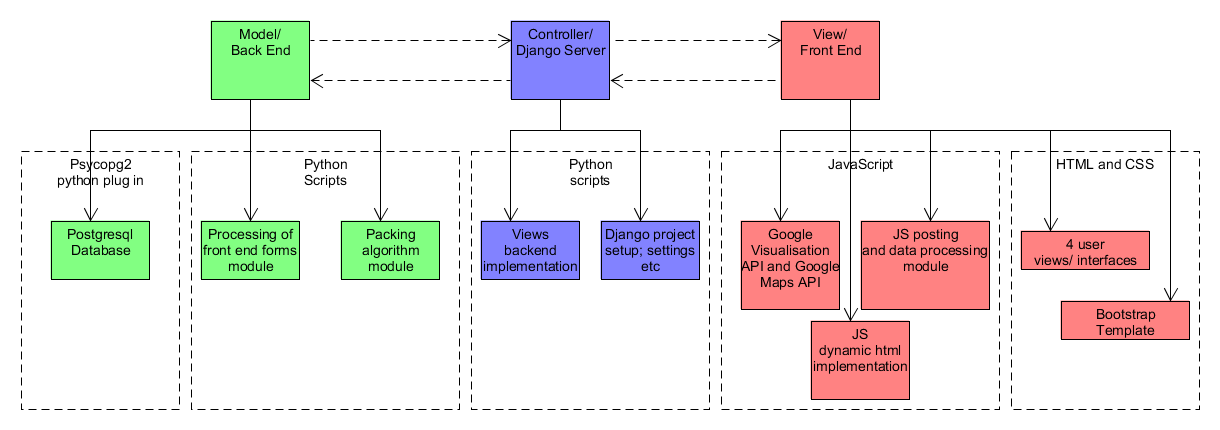
\includegraphics[width=5in]{pictures/system_architecture.png}
\caption{The system architecture}
\label{Architecture}
\end{figure}

\subsection{System Overview}
Figure \ref{SystemDesign} shows an overview of the entire system. It shows how both the front and back end systems interact with each other to form a cohesive system. 
\begin{figure}[hbt!]
\centering
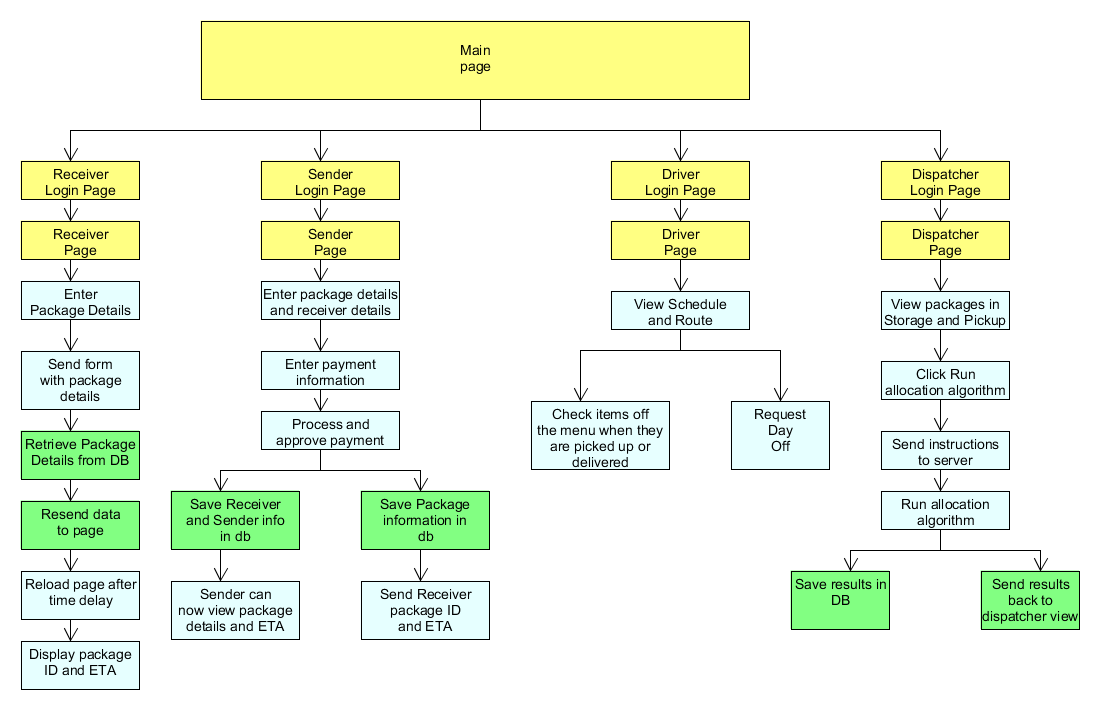
\includegraphics[width=5in]{pictures/system_diagram.png}
\caption{The overall system design}
\label{SystemDesign}
\end{figure}

Figure \ref{PackageLifeCycle} shows the package life cycle from the time the sender requests the package to be picked up to the time the driver delivers it at its' destination.

\begin{figure}[hbt!]
\centering
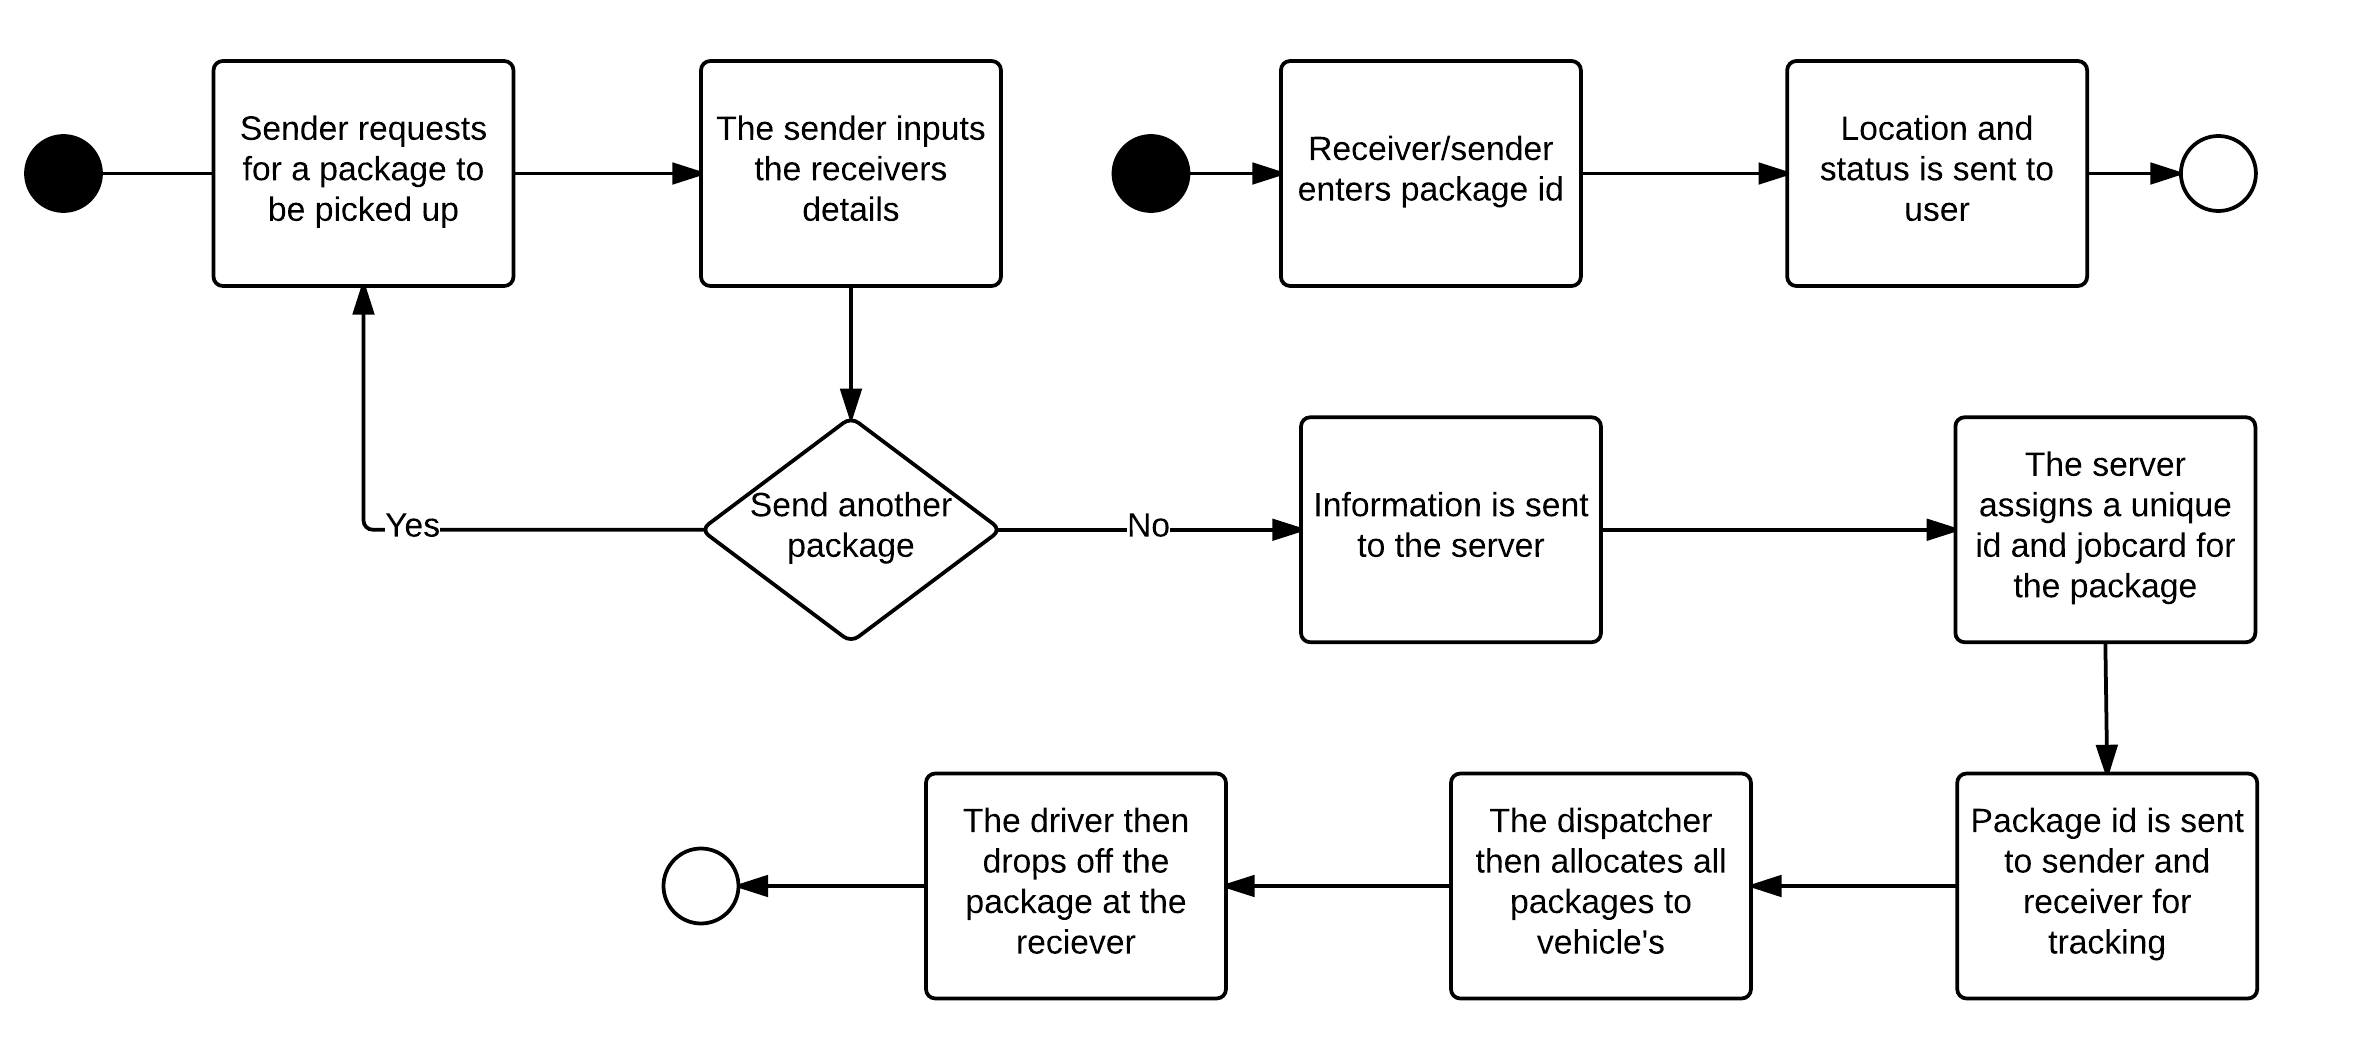
\includegraphics[width=5in]{pictures/package.png}
\caption{The package life cycle}
\label{PackageLifeCycle}
\end{figure}


\subsection{Front-end}
Proper design is important so that teething problems can be avoided which results is a more streamlined and efficient implementation process. The design process also allows a developer to foresee problems before they occur, therefore facilitating upgrades. The first step in the design process is to determine what functionality each user dashboard should preform. The second step would be to use the information found in step one, in order to create a visual representation in the form of dashboards. The final step in the design process is to edit and analyse the dashboards, making sure that there is a good flow, that the content is correct and that the format is correct, ultimately lending to a good customer experience.
\\

The aim of the first step is to correctly identify all the users and their expections from the system. Since each of these users also needs to interact with the system, it is important to identify their goals and give them a means to do this. From this identification, the dashboards can then be designed in a way in which the important information is easily accessible and always visible. By looking at the inputs and outputs of each web-page it is easy to determine whether the functionality defined at the beginning of the process has been achieved.
Table 2.1 summarises this process.
\\


Once the data is collated,the dashboards can then be designed. Each dashboard design will be described below.
\\


The sender view, as seen in Figure \ref{SenderView},is used when a package needs to be sent. The left side of the page allows a user to input the dimensions of a package and the address of the pick-up and drop off points. The right hand side of the page allows the sender to pay for the service and view details of pick-up and delivery times. The information is sent to CourierJZ on submission.
\\

\begin{figure}[hbt!]
\centering
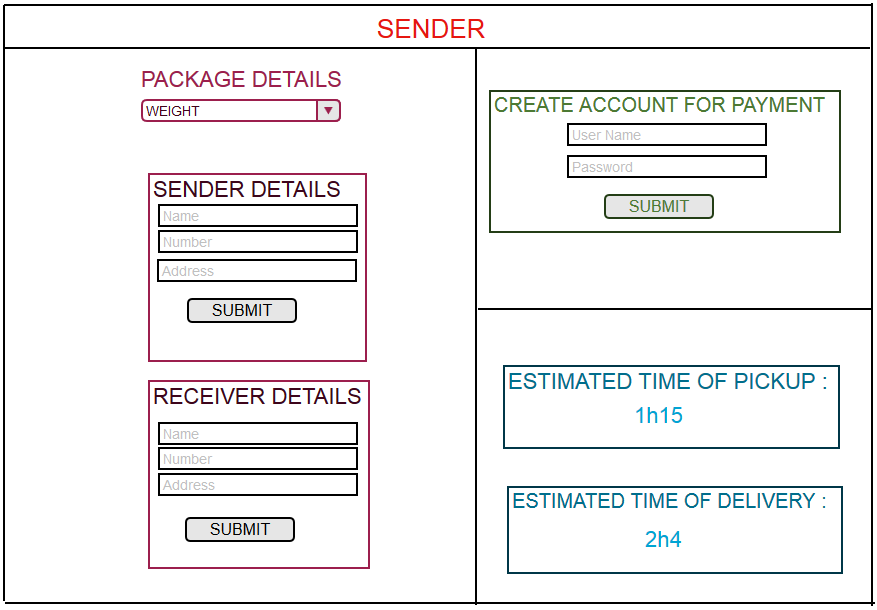
\includegraphics[width=3.5in]{pictures/sender.png}
\caption{The sender view}
\label{SenderView}
\end{figure}


The receiver views, as seen in Figure \ref{receiverBeforeView} and Figure \ref{receiverAfterView}, is used when the receiver wants to track the package being sent to them. The receiver enters the tracking ID and receives the location and status on submission.
\\

\begin{figure}[hbt!]
\centering
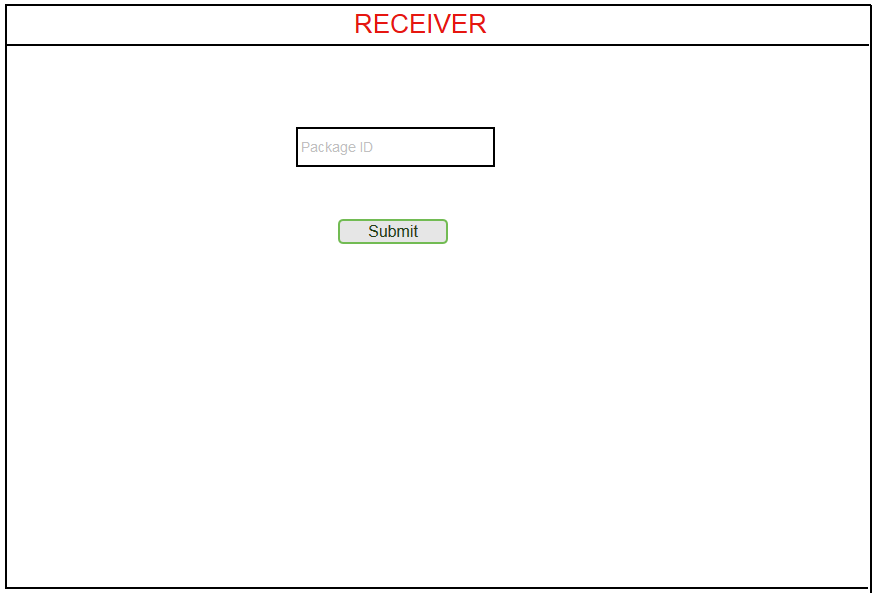
\includegraphics[width=3.5in]{pictures/receiverBefore.png}
\caption{The receiver before view}
\label{receiverBeforeView}
\end{figure}

\begin{figure}[hbt!]
\centering
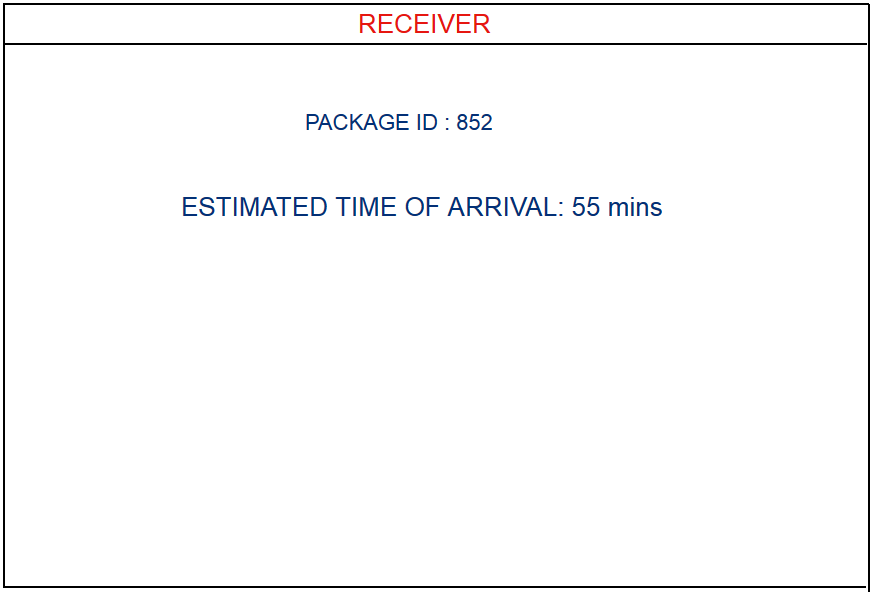
\includegraphics[width=3.5in]{pictures/receiverAfter.png}
\caption{The receiver after view}
\label{receiverAfterView}
\end{figure}

The driver view,as seen in Figure \ref{DriverView}, shows a map of the current location of a driver and the destination point of the current package being delivered or picked up. These destination points change as each pick-up/delivery is made. The contact details and estimated time of arrival of each client is also displayed on screen. This information is essential in order for the driver to perform their duties.
\\


\begin{figure}[hbt!]
\centering
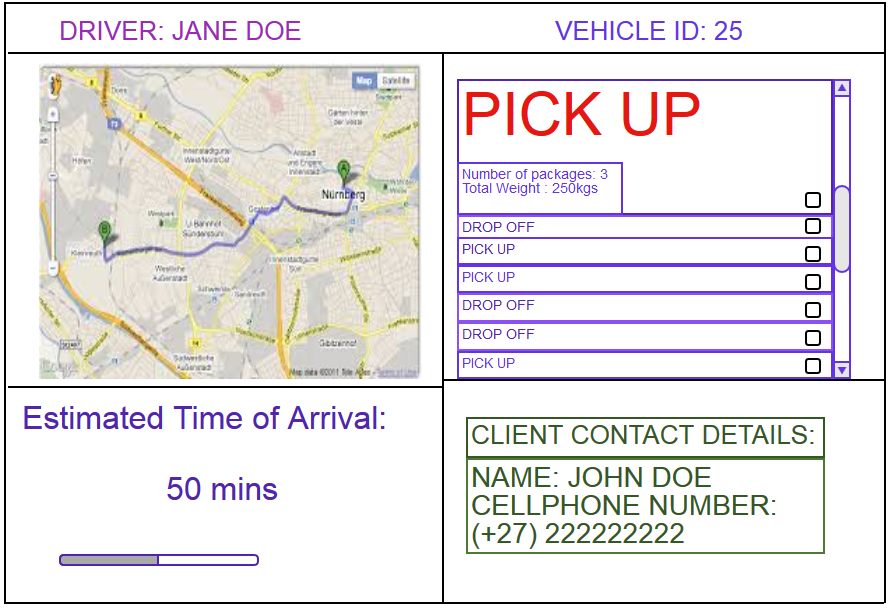
\includegraphics[width=3.5in]{pictures/driver.png}
\caption{The driver interface}
\label{DriverView}
\end{figure}

The dispatcher view, as seen in Figure \ref{DispatcherBefore}, provides details on both packages in storage and requested for pick-up. The run-allocation algorithm button performs scheduling for items in storage to be dispatched and schedules the items for pick-up. 
\\

\begin{figure}[hbt!]
\centering
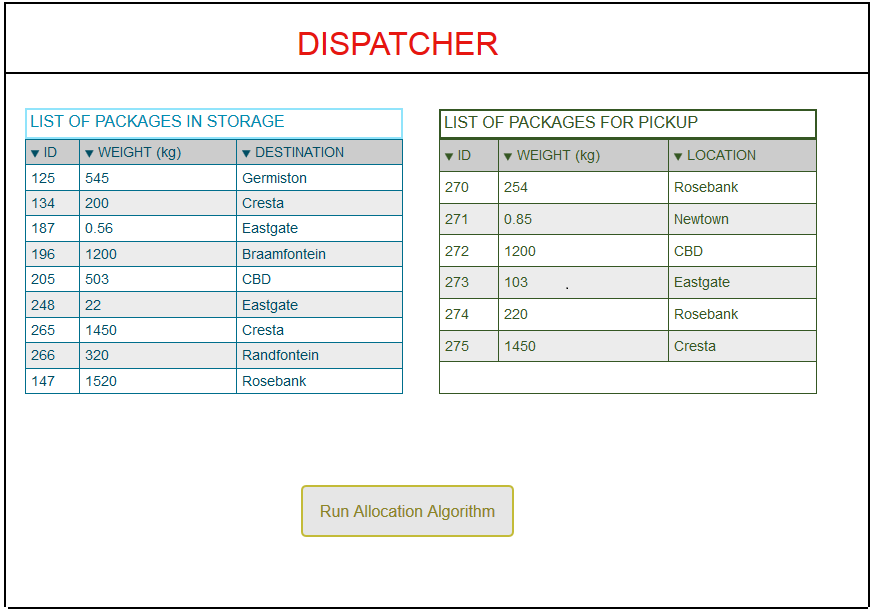
\includegraphics[width=3.5in]{pictures/dispatcherBefore.png}
\caption{The dispatcher view}
\label{DispatcherBefore}
\end{figure}

The CEO view, as seen in Figure \ref{CEOView}, allows the CEO to request various reports summarising the operations of CourierJZ and view them on the right side of the page.
\\

\begin{figure}[hbt!]
\centering
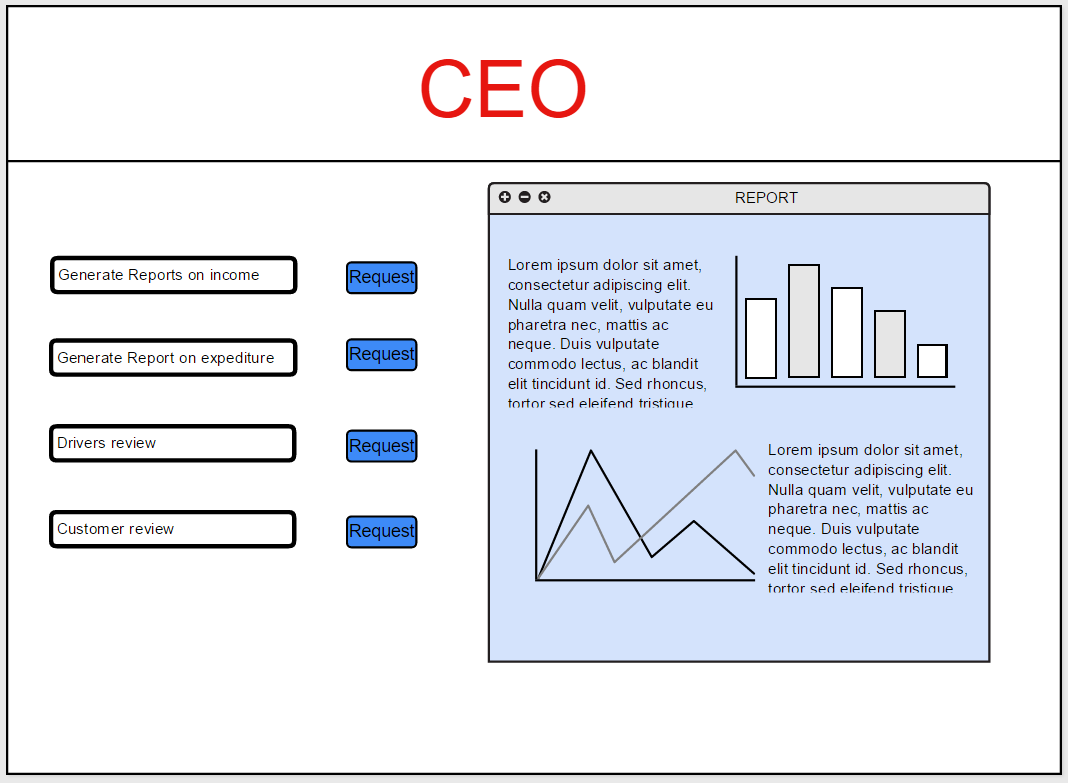
\includegraphics[width=3.5in]{pictures/CEO.png}
\caption{The CEO view}
\label{CEOView}
\end{figure}

manager
\\

\begin{figure}[hbt!]
\centering
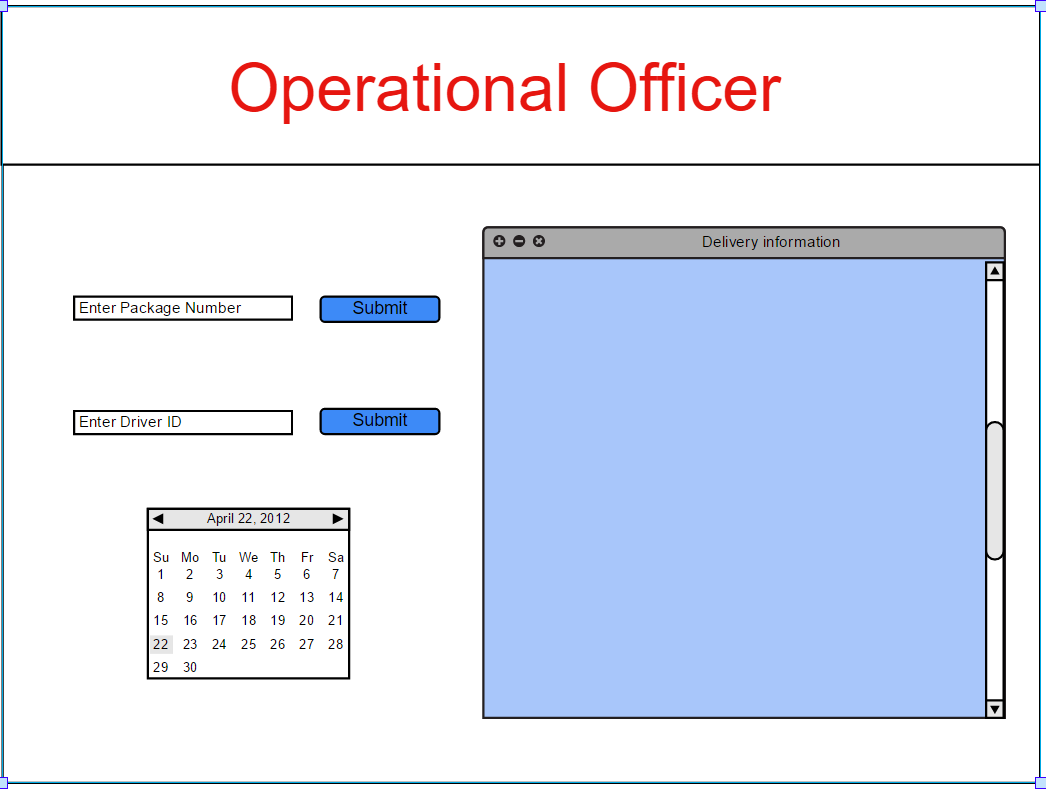
\includegraphics[width=3.5in]{pictures/operational_officer.png}
\caption{The operations officer view}
\label{OperationsView}
\end{figure}

The operational officer view, as seen in figure \ref{OperationsView} allows the officer to respond to calls from clients and drivers. The officer can enter either the truck id or the tracking id in order to receive the relevant information on it. 
\\

\begin{figure}[hbt!]
\centering
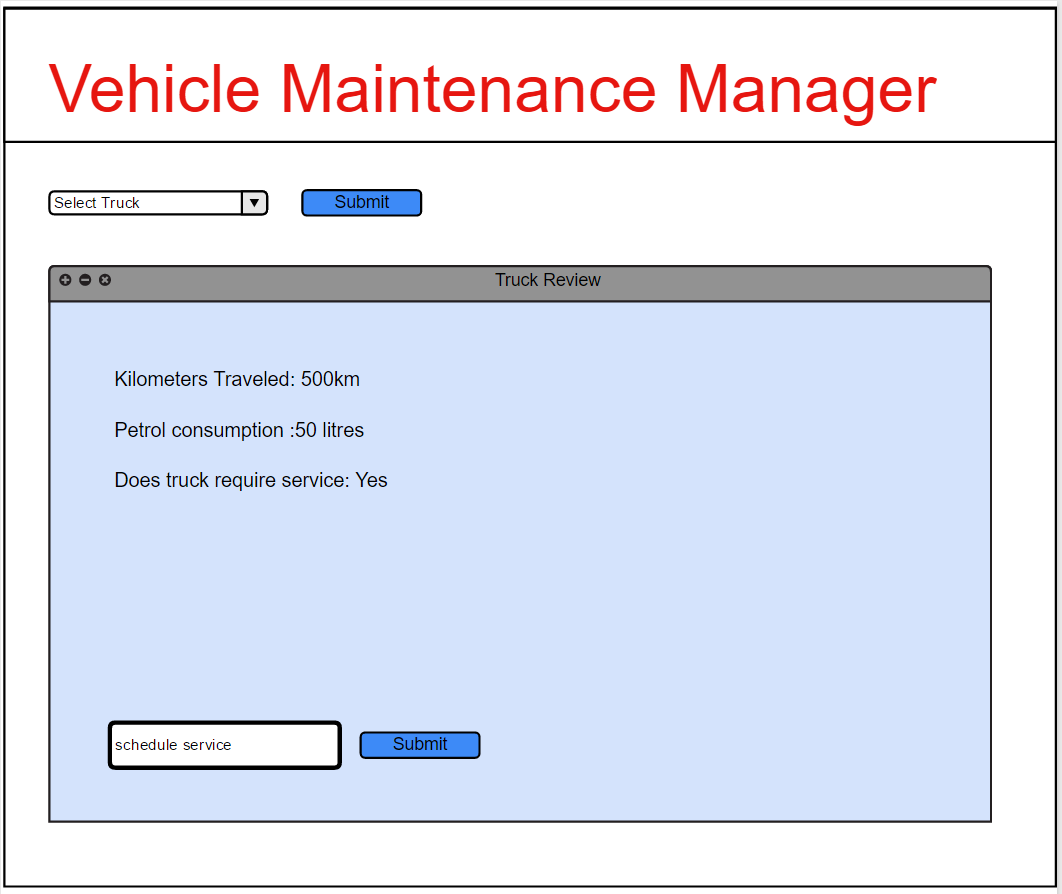
\includegraphics[width=3.5in]{pictures/maintenance.png}
\caption{The maintenance view }
\label{MaintenanceView}
\end{figure}

The system administrator view, as seen in Figure \ref{AdminView}, allows the manager to make updates to the system. The manager can start,stop and select a file from which a update must occur. The manager can also view a list of when back-ups on the system were performed and request that a back-up be currently performed.
\\

\begin{figure}[hbt!]
\centering
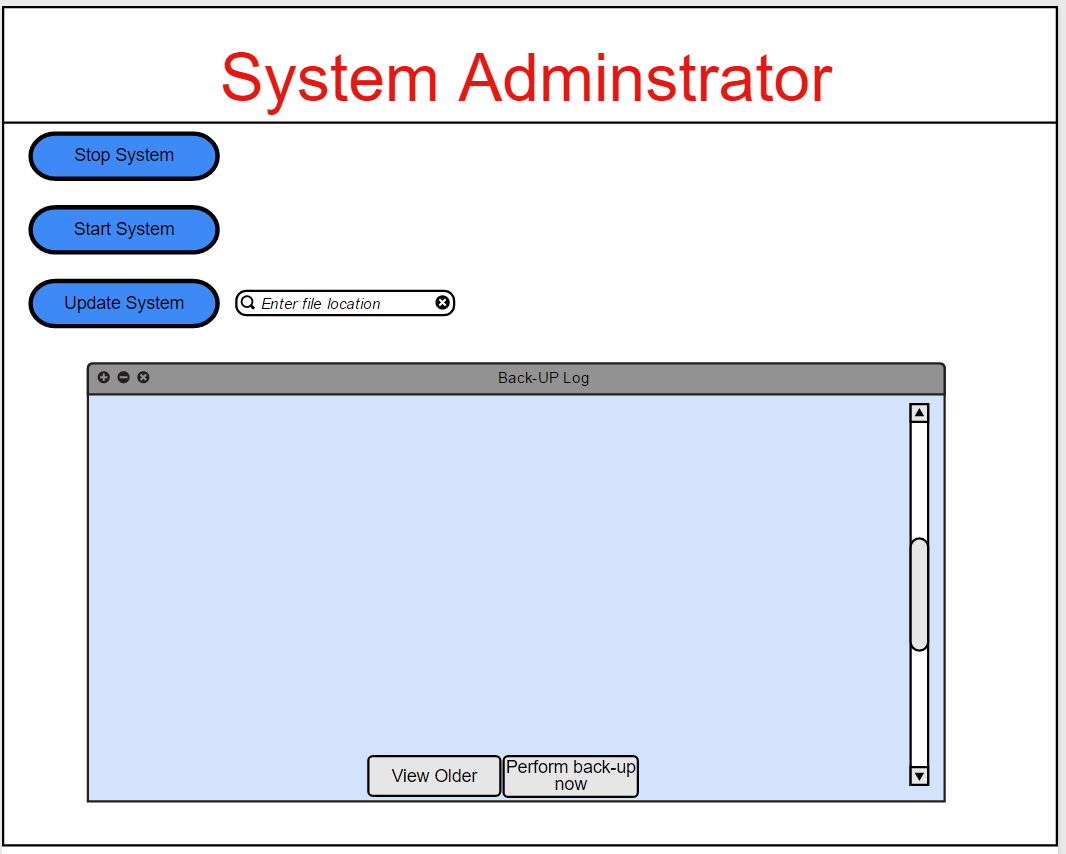
\includegraphics[width=3.5in]{pictures/admin.png}
\caption{The system administrator view}
\label{AdminView}
\end{figure}

The accounts officer view,as seen in Figure \ref{Accounts}, allows the accounts officer to select a time period and then export the accounts information to an accounting software such as PASCAL in order to perform the necessary inspections or calculations.
\\

\begin{figure}[hbt!]
\centering
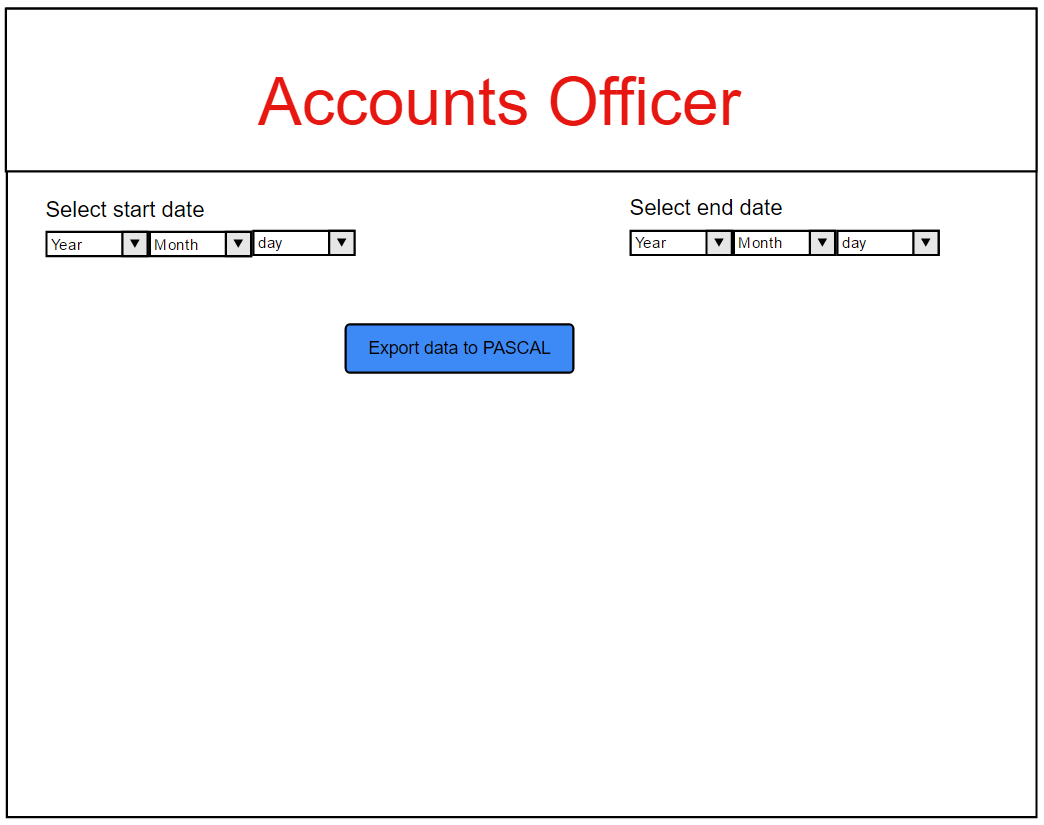
\includegraphics[width=3.5in]{pictures/accounts.png}
\caption{The accounts officer view}
\label{Accounts}
\end{figure}

As can be seen from the web designs, the information is placed in a  logical order that gives the user an intuitive experience. The webpages only provide the necessary information for the task and does not add excess information. The webpages also avoid the use of contrasting colours and instead used complementary colours to provide a ergonomic user experience. The colours were restricted to blue, purple, red and some grey. A white background was chosen in order to create a high contrast to the predominately black writing with a simple font, improving readability.  


\begin{table}[]
\centering
\caption{Responsibilities and activities of relevant users}
\label{my-label}
\begin{tabular}{|p{2cm}|p{4cm}|p{4cm}|p{4cm}|}
\hline
\textbf{Webpage}            & \textbf{Responsibilities}                                                                           & \textbf{Input}                     & \textbf{Output}                                          \\ \hline
Main                        & Provide a page for all users to select their role                                                   & Type of user                       & Correct user login page                                  \\ \hline
Login                       & Provide a page to verify user credentials                                                           & User email,                        & Correct user dashboard                                   \\ \hline
                            &                                                                                                     & User password                      &                                                          \\ \hline
Sender                      & Provide a page for a sender request for a package to be picked up from their location and delivered & Package dimensions                 & Delivery cost                                            \\ \hline
                            &                                                                                                     & Receiver details                   & Create a delivery job card for CourierJZ                 \\ \hline
Receiver                    & Provide a page for a receiver to view the delivery details of the package                           & Tracking number                    & Package location and status                              \\ \hline
Driver                      & Provide a page for the driver to view a map and details of all deliveries and pick ups              & Checklist for pickup or delivery   & Update server on package status                          \\ \hline
Dispatcher                  & Provide a page to view all packages and their locations                                             & Initiation of allocation algorithm & Update server on where package status                    \\ \hline
CEO                         & Provide a page to view operational activities and data analysis                                     & Reports to be generated            & Generate reports on server and return to webpage         \\ \hline
Operational Officer         & Provide a page to view details on all clients and drivers                                           & Driver or client details           & Information for respective driver or client              \\ \hline
Vehicle maintenance officer & Provide a page to view information on all vehicles                                                  & Vehicle id for maintenance         & Add vehicle to schedule for maintenance                  \\ \hline
System admin                & Provide a page to view system status and maintenance                                                & Pause or start the system          & Initiate the action to pause or start                    \\ \hline
                            &                                                                                                     & Request for system backup          & Pause the system, do backup, then start the system again \\ \hline
Accounts officer            & Provide a page to view all financial information                                                    & Request financial information      & Display financial information                            \\ \hline
\end{tabular}
\end{table}

\subsection{Back-end}
\begin{figure}[hbt!]
\centering
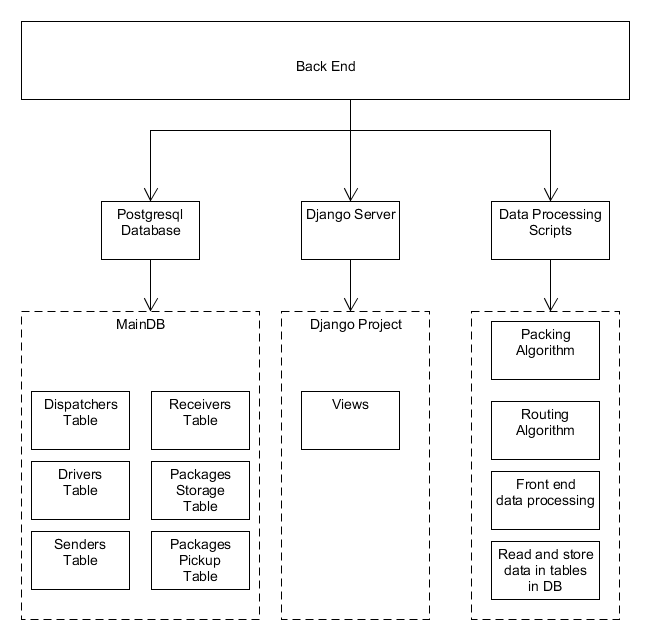
\includegraphics[width=3.5in]{pictures/backend.png}
\caption{The backend system diagram}
\label{Backend}
\end{figure}

Figure \ref{Backend} shows the entire back-end system design. The system has been categorised into 3 parts; the postgresql database, the django server and the data processing scripts. 

\subsubsection {The postgresql database - designing the database}
Due to the nature of vehicle management systems data, a relational database has been selected. The database will be used to store all the information relevant to the operation of CourierJZ. This information includes client information, staff information, package information, vehicle information and financial information. The data should be organised in a manner that is easy to access. 
\\

No data has been provided therefore dummy data has to be generated. The data is generated from the site www.generatedata.com which allows you to generate test data 100 rows at a time. Receiver, sender, dispatcher and driver dummy data has been generated.
\\

The data will be stored in tables. This requires creating primary keys for each of the rows generated. This will ensure that each row in a table will be unique. Figures \ref{First}, \ref{Second} and \ref{Third} show the tables designed. The tables are a receiver, sender, driver, serviceclientlist, dispatchers and packages tables. The variables in red are the primary keys. The purple variables are foreign keys. The foreign keys link the various tables. 
\\ 

\begin{figure}[hbt!]
\centering
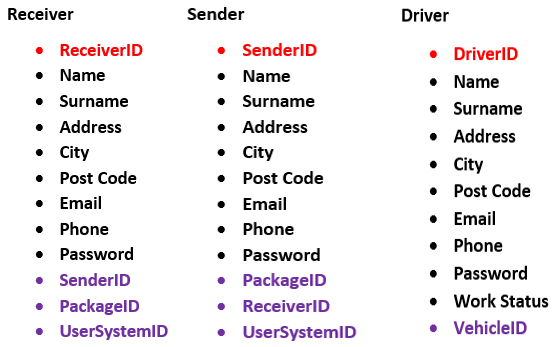
\includegraphics[width=3.5in]{pictures/db/first3.png}
\caption{The receiver, sender and driver tables}
\label{First}
\end{figure}


\begin{figure}[hbt!]
\centering
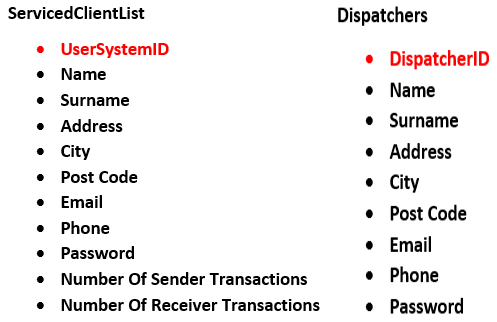
\includegraphics[width=3.5in]{pictures/db/second2.png}
\caption{The servicedclientlist and dispatchers tables}
\label{Second}
\end{figure}

\begin{figure}[hbt!]
\centering
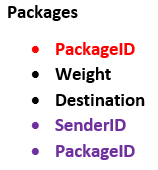
\includegraphics[width=1.5in]{pictures/db/last1.png}
\caption{The packages table}
\label{Third}
\end{figure}

\subsubsection{Views}
Views are implemented in the controller in views.py. They connect the database and the front end. Functions are implemented in the views that are tied to a url. A view function, is a Python function that takes a Web request and returns a Web response. When a user enters a url that function is called. Each function specifies an html that will be opened when the url is entered. 
\\

The functions implemented are the sender, dispatcher, receiver, driver, main, login\_sender, login\_receiver, login\_driver, login\_ceo and login\_dispatcher. The first 4 views receive posts from the front end. User authentication occurs and the response is sent back to the front end. 
\\

\subsubsection{Data Processing Scripts}
\textbf{Algorithms}\\
Two algorithms should be implemented in order to service the needs of the dispatcher, sender and the driver. The route and vehicle that a driver chooses is determined by application of a vehicle routing algorithm. To determine which vehicle parcels should go into a packing algorithm should be implemented. \\ 


\underline{Routing Algorithm} \\
Determining the route that a driver has to take can be labelled as a transportation model problem \cite{Psraftis}. As noted in \cite{Ichoua} these problems can fall into one of two categories, static and dynamic. In the static scenario all the data is known before the routing takes place and does not change once it has. In the dynamic case, all or some of the data is only received as the route calculation is taking place. The information can still change even after the routing process has been applied \cite{Madsen} .\\ 

Static routing problems include the time-dependent travelling salesman problem (TSP) and the probabilistic TSP. In  the time-dependent TSP, travelling times between nodes are not constant but change through time in a known manner. For the probabilistic TSP, travel times are deterministic but demand at each node occurs with a known probability, \textit{p} \cite{Psraftis}.\\

At present it should be noted that determining a route a driver should take, a slew of dynamic algorithms may be used. These include dynamic routing, dynamic shortest paths, dynamic traffic assignment, dynamic fleet management and dynamic facility location \cite{Psraftis}. Dynamic routing can be applied to multiple contexts including courier services and combined pickup and delivery services as demonstrated by Psaraftis in \cite{Psraftis}. \\


\underline{Packing Algorithm} \\

There are a number of ways which one can implement a packing algorithm; these algorithms are commonly called bin packing algorithms. Some of the most common algorithms are; First fit algorithm, next fit, best fit algorithms and there are different variations of these algorithms based on the application. A general simple case of a first fit bin packing algorithm is when there is a limited number of bins of predetermined size and a queue of items that are going to be fitted in the bin. You allocate an item based on where it will fit first while traversing the bins, however this could result in a waste of space (since you could assign one big item to a space that would fit two small item and that could have increased the efficiency if the aim was to package as many packages as possible in the given bins) \cite{Hong}. With the next fit algorithm, the first fit algorithm is used to allocate the first item, thereafter instead of starting from the first bin to allocate the rest of the item, you move on to the next bin that has space if the current bin cannot accommodate the item. The best fit bin packing algorithm traverses all the bins and puts the items in the bin that has the space that best suit the items dimensions \cite{Zhu}. The best fit algorithm takes a longer while than the other algorithm because it has to traverse the bin searching for a best fit and comparing before allocating any item to a bin \cite{Huang}. All these packing algorithms can be implemented in one, two or three dimensions, and weight can be added as the fourth dimension if the packages are matter.  Increasing the dimensions increases the complexity and run time of the algorithm. \\

The design approach followed for the design of the packing algorithm is a combination of the 3 basic algorithms that were mentioned in the literature review and an addition of a few basic functionalities. The assumptions made when designing the algorithm was there will be no package that will exceed the dimensions of the truck, and all trucks are of equal dimensions. The algorithm is made up of four lists; a list of all the trucks and a queue of packages. Each package is an array in which, the first, second, third, and fourth elements are the package’s identifier, its height, width and length respectively. The first   package will chosen based on the furthest delivering distance from the store house. Thereafter the following packages will be sorted relative to the delivery distance of the first package while obeying the rules of the best fit algorithm. This particular design was chosen because even if we might not be able to pack the truck with the most goods, it solves the travelling sales man problem and it brings about efficiency in the system. The best fit algorithm is a very expensive algorithm in terms of runtime. And combining it with methods to calculate the distance between the last element and the next element to append is going to be cost even more runtime. Thus the trade-off of this design is that for big data sets it might be slow.



  

\subsection{Use Cases}
\begin{itemize}
\item Send a package \\
Primary Actor: \quad \quad Sender \\
Scope:		\quad \quad	 Package allocation system \\
Stakeholders and Interests: \\
Sender - wants to send package as fast as possible and as cheap as possible \\
CourierJZ - wants package information, delivery details and pricing information \\
How do you perform the action: \\
\begin{itemize}
\item Create an account if you do not have one
\item Visit home page and login
\item Enter package dimensions and relevant information
\item View pricing to see affordability
\item Enter destination details
\item Submit information and make payment
\end{itemize}

\item Receive a package\\

Primary Actor: \quad \quad Receiver \\
Scope:		\quad \quad	Delivery time estimation system and Package tracking system  \\
Stakeholders and Interests: \\
Receiver - wants date and time of delivery of the package, and wants to know where the package is. \\
CourierJZ - wants the contact details of the receiver \\
How do you perform the action: \\
\begin{itemize}
\item Upon reception of the payment from the sender, the receiver receives an email notifying them of the delivery
\item The email posses a link to the website and a package identity number that the receiver can use to view the estimated time of arrival of their parcel and where their parcel is.

\end{itemize}


\item Get work schedule and route\\

Primary Actor: \quad \quad Driver \\
Scope:		\quad \quad	 Route allocation system \\
Stakeholders and Interests: \\
Driver - wants to be allocated a vehicle and a route to commence with delivering \\
CourierJZ - wants to effectively allocate vehicles to drivers with efficient route to follow \\
How do you perform the action: \\
\begin{itemize}
\item Driver signs into the system
\item Details of the allocated vehicle and route are displayed 
\end{itemize}

\item Request day off\\

Primary Actor: \quad \quad Driver \\
Scope:		\quad \quad	Human resources management system, route and package allocation systems  \\
Stakeholders and Interests: \\
Driver - wants to be given a day off \\
Dispatcher - cannot allocate routes and a vehicle to a driver who has requested a day off \\
How do you perform the action: \\
\begin{itemize}
\item Log into page the driver page
\item Click the request day off button available on page
\item Choose the day you want to take off from the resulting calendar view
\item Submit selection and await confirmation 
\end{itemize}

\item Run a scheduling module\\

Primary Actor: \quad \quad Dispatcher \\
Scope:		\quad \quad	Route allocation system and package allocation system  \\
Stakeholders and Interests: \\
Dispatcher - wants to allocate routes to drivers and decide which trucks packages can go into \\
Sender - wants their parcel picked up and eventually delivered as soon as possible \\
Driver - wants to choose a route and vehicle from allocated routes and vehicles \\
How do you perform the action: \\
\begin{itemize}
\item The driver logs into the their page
\item The driver clicks the request day off button available on their page
\item The driver will choose the day they want off from the resulting calendar view 
\item The driver will then submit their selection and await confirmation 
\end{itemize}

\item Schedule a vehicle for service\\

Primary Actor: \quad \quad Vehicle maintenance manager \\
Scope:		\quad \quad	Maintenance scheduling  \\
Stakeholders and Interests: \\
 Clients: They want to know that the service is reliable and trustworthy\\
 Driver: they need vehicles to be safe and available\\
 CourierJz: They want to ensure that vehicles will not breakdown\\
 Government: they want to ensure that all vehicles are roadworthy\\
How do you perform the action: \\
\begin{itemize}
\item View vehicles details on the vehicle maintenance manager page
\item Determine if the vehicle needs maintenance by following the manufactures guidelines
\item If the vehicle is due for maintenance then press the submit
\end{itemize}

\item Back up and maintain system\\

Primary Actor: \quad \quad System Admin \\
Scope:		\quad \quad	 System Maintenance \\
Stakeholders and Interests: \\
Clients: They want a system that is smooth and easy to use \\
CourierJz: They want a system that if free of problems \\
How do you perform the action: \\
\begin{itemize}
\item The system administrator must log on to their page
\item They can then view the backup log
\item Should a backup be required, they can then opt to perform a backup
\end{itemize}

\item Accounts auditing\\

Primary Actor: \quad \quad Account Officer \\
Scope:		\quad \quad	Accounts system  \\
Stakeholders and Interests: \\
Account holders- He/She wants to make sure that the he/she has been charged the 
                                        correct amount. \\
Account officer-A list of all the accounts which have made payments in a period of time   
                                    that is being audited. \\
How do you perform the action: \\
\begin{itemize}
\item Account officer logs in to the accounts page.
\item Select the time period he/she wants to audit
\item Press button which says export to accounting software.
\end{itemize}


\item Carry out operational checks and data analytics\\

Primary Actor: \quad \quad CEO \\
Scope:		\quad \quad	JZ Courier  \\
Stakeholders and Interests: \\
CEO- wants to get an overview of how the company performing \\
How do you perform the action: \\
\begin{itemize}
\item  CEO logins into the CEO page
\item CEO clicks button to determine what report/statistics he/she would like to view
\item Report appears in a window on the page 
\end{itemize}


\end{itemize}


\section{Relevant Modules Description / Results}

\subsection{Front-end}
The implemented webpages are shown below, these webpages show how the design of the pages have changed from their initial stages to their implementation stages. The company logo and any unnecessary of user implementations have been left out of these pages as the focus was to create a user friendly page first, with changes added later to further identify the company and cement the company image in the design image. The webpages are designed from a bootstrap templates which consist of HTML, CSS and JavaScript code. This code was then modified to get the webpages below.

\begin{figure}[hbt!]
\centering
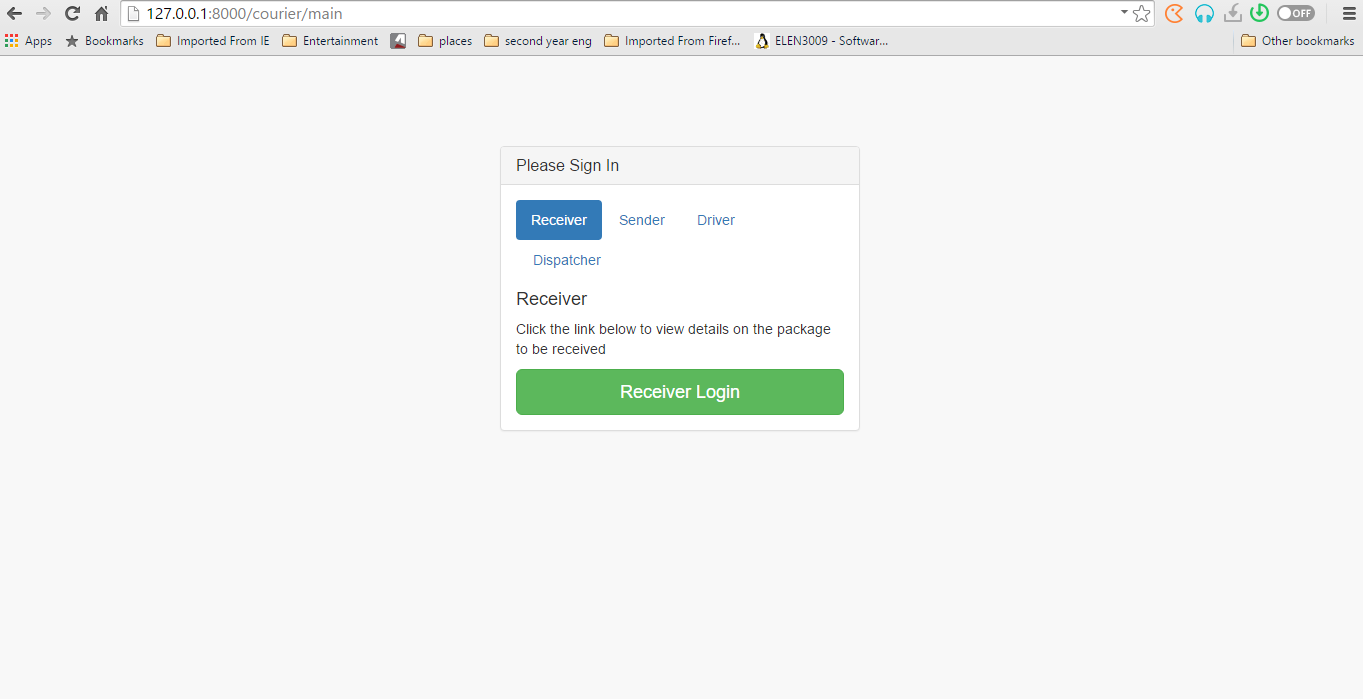
\includegraphics[width=3.5in]{pictures/main_page.png}
\caption{The main page - the first page a user goes to}
\label{MainPage}
\end{figure}

The above page shows the main page that every user must access before they can access their dashboard. This page is important in the prototype stage as it offers a centralized location where all users can interact and access their user specific page. In this page the user is able to click on their designation (i.e. receiver or driver) and see a short description of their role in the CourierJZ ecosystem. Once they have picked their designation, they can then access the specific login page for their user dashboard. This page also assists in troubleshooting as when the system administrator logs out of one user dashboard they are brought back to this page and can then proceed to the next user dashboard. The login section will be described below.

\begin{figure}[hbt!]
\centering
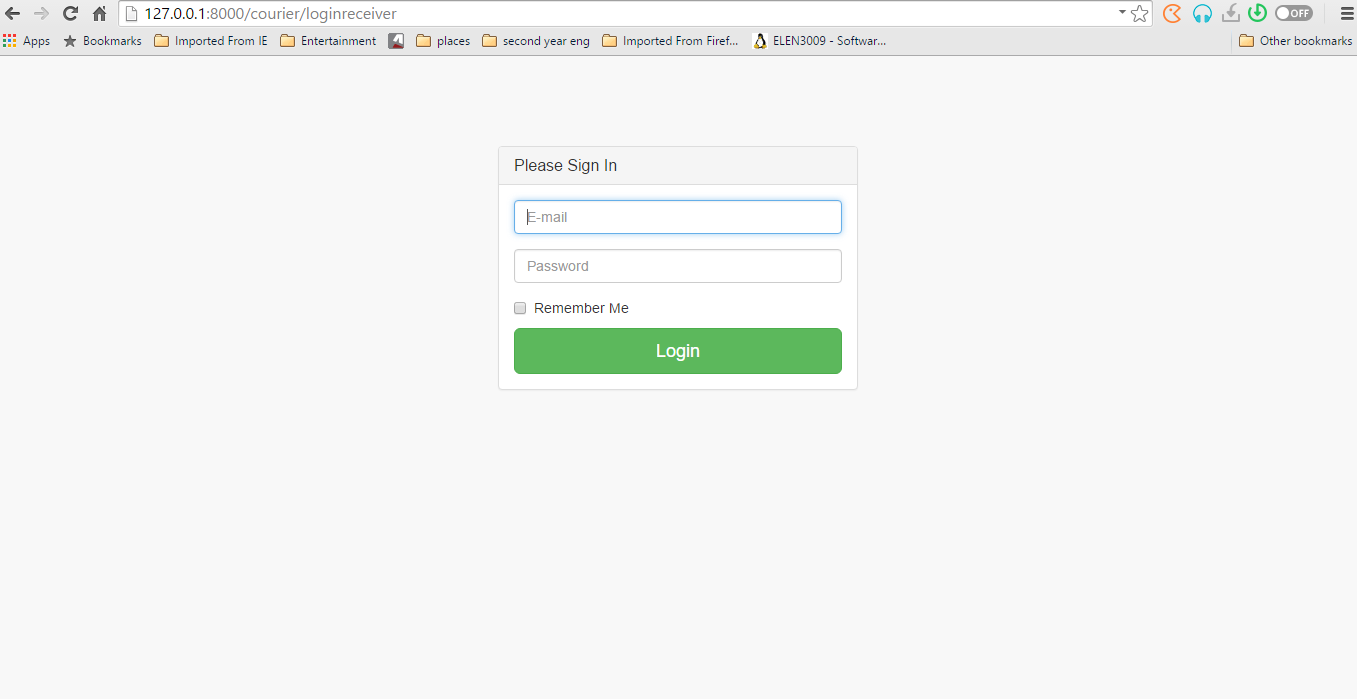
\includegraphics[width=3.5in]{pictures/loginreceiver_page.png}
\caption{The login page of the receiver}
\label{LoginReceiverPage}
\end{figure}

The user is brought to a specific login page based on the designation they picked on the main page. This page facilitates the login to their user specific dashboard. In the current prototype there is only one login and password for each designation.  When they enter their details and submit they are taken to their user dashboard. On this dashboard a welcome notification will pop up if the username and password was correct and subsequently display all the dashboard information, should the login details be incorrect then a pop up say such will be displayed and the user will be taken back to the login page

\begin{figure}[hbt!]
\centering
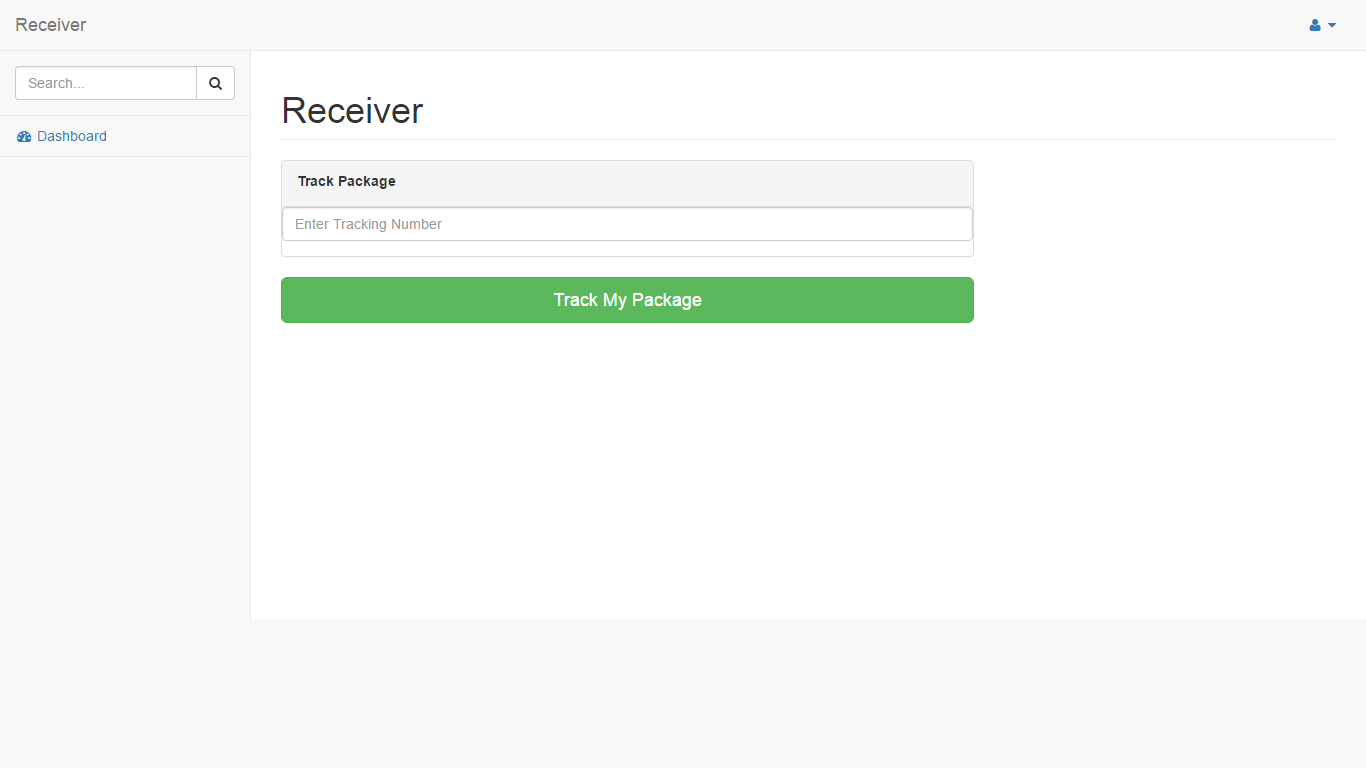
\includegraphics[width=3.5in]{pictures/receiver_page.png}
\caption{The receiver page}
\label{ReceiverPage}
\end{figure}

The receiver dashboard is the simplest of the four implemented dashboards and can be seen as such. This dashboard only has one form with one textbox for submission. Here the user is able to enter their tracking id and submit. On submission a dialogue box will appear that shows the user the location and status of the package

\begin{figure}[hbt!]
\centering
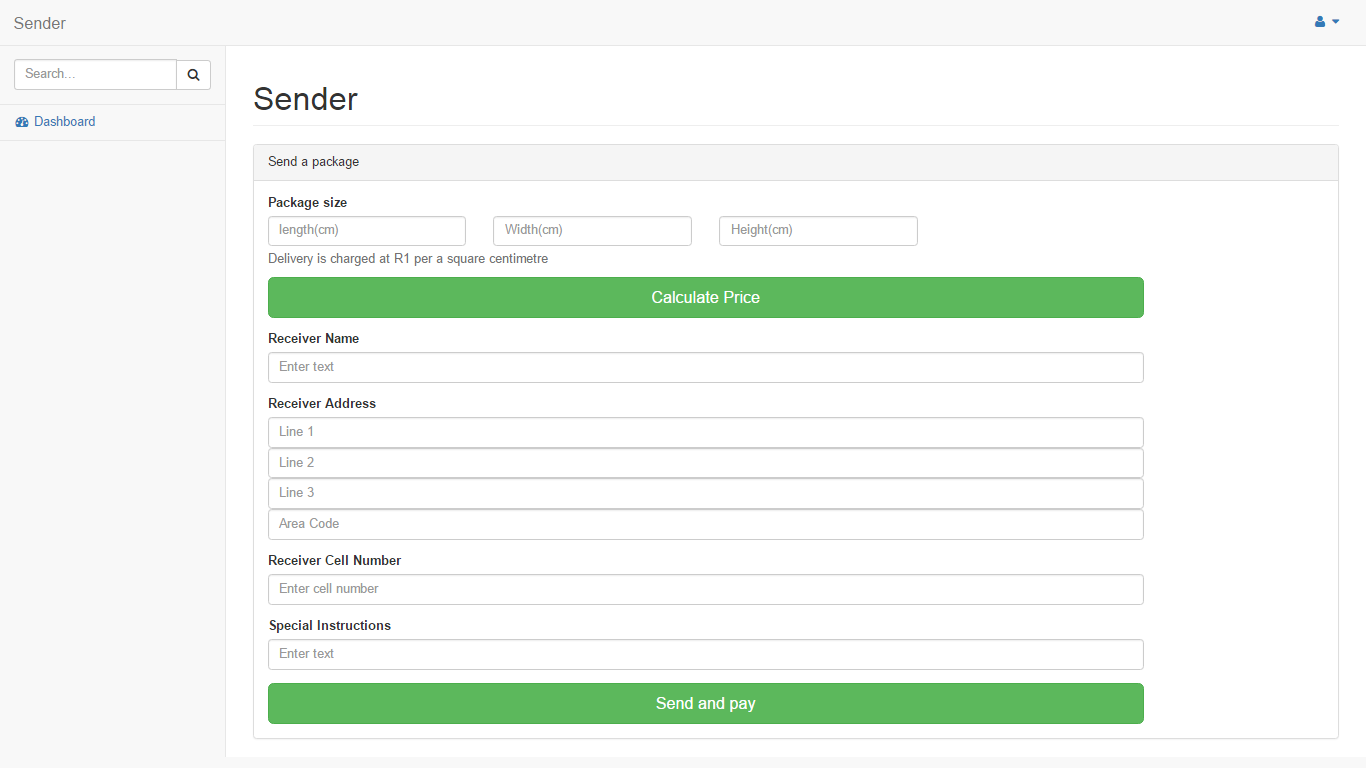
\includegraphics[width=3.5in]{pictures/sender_page.png}
\caption{The sender page}
\label{SenderPage}
\end{figure}

The sender page is basically the heart of CourierJZ as without this page, the business would not exist. This page consists of one form and two buttons. The first button allows the user to get the price of sending the package by inputting its dimensions. The user can then decide if sending the package is still feasible before further entering the receiver's details. If the user chooses to proceed and enter the receiver's details they can then submit which will send a jobcard to courierJZ's servers to process. This process is further streamlined since the user had entered their details when they created their profile page(This was not implemented in the prototype stage). This means that the users address will already be saved in the database and that payment will be automatic.

\begin{figure}[hbt!]
\centering
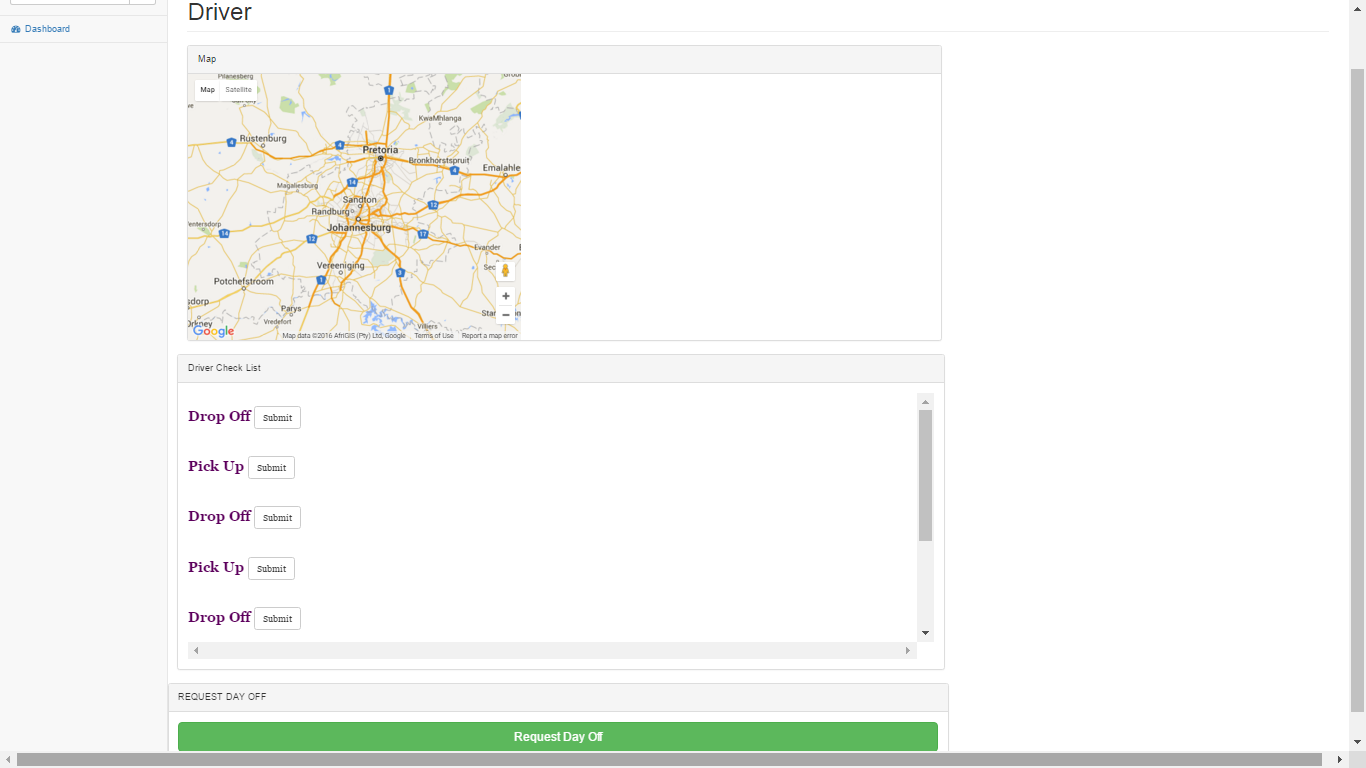
\includegraphics[width=4.5in]{pictures/driver_page.png}
\caption{The driver page}
\label{DriverPage}
\end{figure}

The driver page consists of two sections. The first section contains a map and the second section contains information of the locations to be visited. The map shows the current location of the driver and the destination of the current package to be delivered. This helps the driver find the shortest possible route to the destination as it uses the google maps API which combines the route data with crowdsourced traffic data. The second section provides the driver with the locations and details of each client. This includes the contact information and whether the client has a package to be picked up or needs one to be delivered. Once to location has been visited and the appropriate action is taken, the driver may then update the server by pressing the update button.


\begin{figure}[hbt!]
\centering
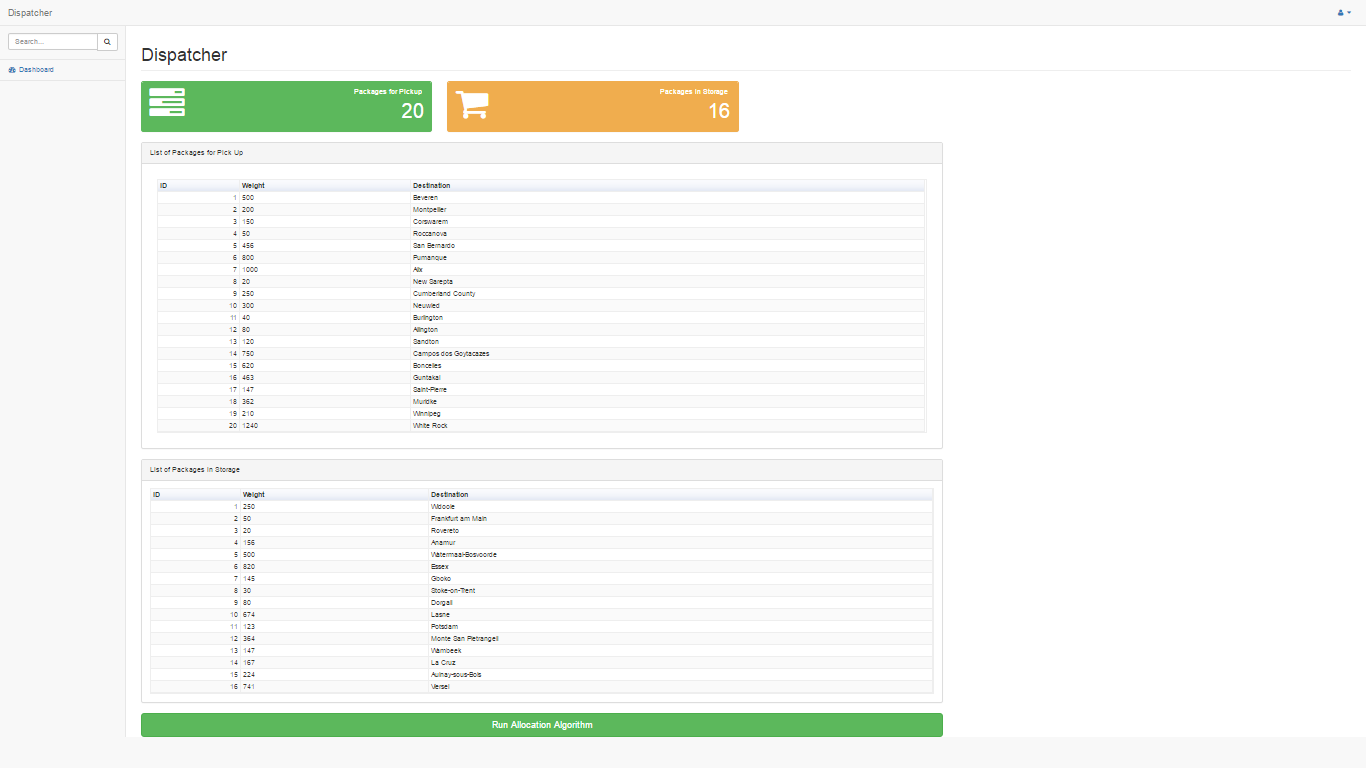
\includegraphics[width=4.5in]{pictures/dispatcher_page.png}
\caption{The dispatcher page}
\label{DispatcherPage}
\end{figure}

The implemented dispatcher dashboard is shown above. This consists of two sections where the dispatcher has access to all the packages in storage and all the packages requested for pick up. The dispatcher may then press the run allocation algorithm, this algorithm determines what each driver will be doing for the day and what packages they are responsible for.

\subsection{Back end}

\subsubsection{Database Tables}
The foreign keys have not been implemented in any of the tables given below. This is because of two reasons, firstly, when the dummy data was being created each of the rows in each table was given primary keys that start from 1 to the number of rows. This means that the primary keys for all tables are in the same range. This means that some foreign keys would have been identical to the primary key. Creating foreign keys would have required linking all the relevant tables in the dummy data. This will have been a time consuming process hence it is not carried out. 

Figure \ref{DispatcherTable} shows the dispatcher table implemented and stored in MainDB, because of the foreign keys that have not been included. 
\begin{figure}[hbt!]
\centering
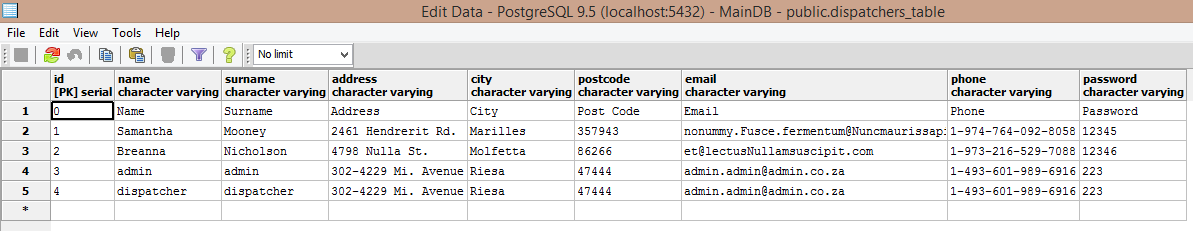
\includegraphics[width=3.5in]{pictures/screenshots/dispatchersdbscreen.png}
\caption{The dispatcher table}
\label{DispatcherTable}
\end{figure}

Figure \ref{DriversTable} shows the drivers table implemented and stored in MainDB. 
\begin{figure}[hbt!]
\centering
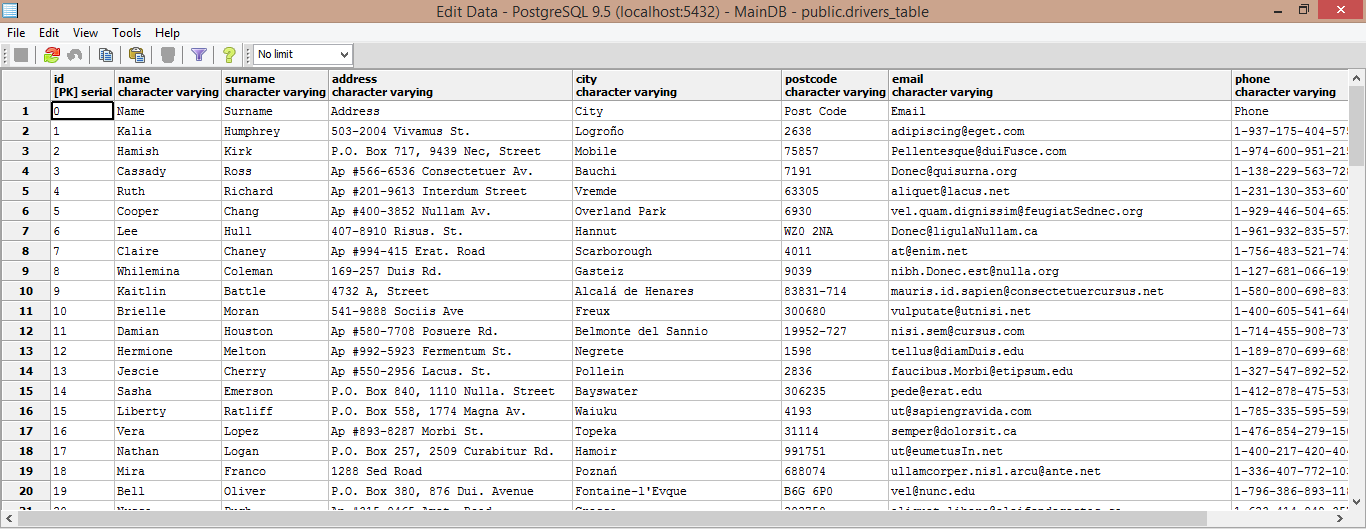
\includegraphics[width=3.5in]{pictures/screenshots/driversdbscreen.png}
\caption{The drivers table}
\label{DriversTable}
\end{figure}

Figure \ref{PackagePickupTable} shows the packages in the pickup table in MainDB.
\begin{figure}[hbt!]
\centering
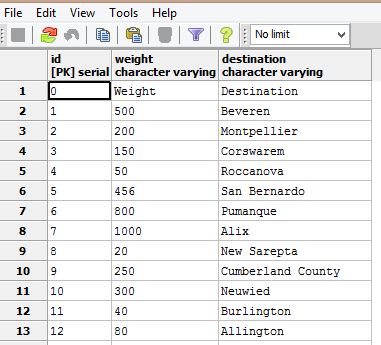
\includegraphics[width=3.5in]{pictures/screenshots/packagespickupscreen.png}
\caption{The packages in the pickup table}
\label{PackagePickupTable}
\end{figure}

Figure \ref{PackageStorageTable} shows the packages in the storage table in MainDB.
\begin{figure}[hbt!]
\centering
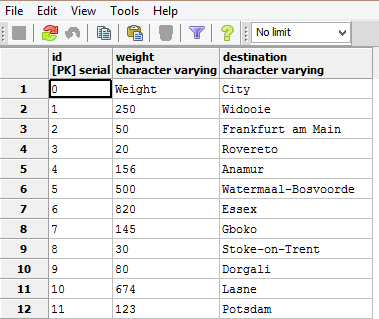
\includegraphics[width=3.5in]{pictures/screenshots/packagesstoragescreen.png}
\caption{The packages in storage table}
\label{PackageStorageTable}
\end{figure}

Figure \ref{ReceiversTable} shows the receivers table created in MainDB.
\begin{figure}[hbt!]
\centering
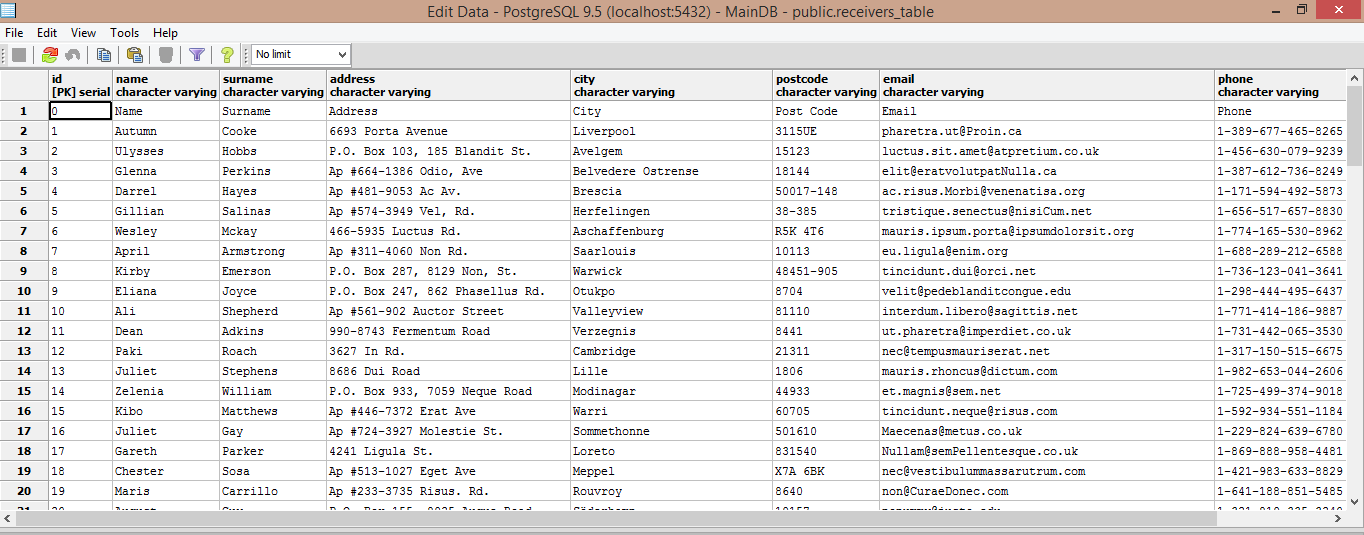
\includegraphics[width=4.5in]{pictures/screenshots/receiversscreen.png}
\caption{The receivers table}
\label{ReceiversTable}
\end{figure}

Figure \ref{SendersTable} shows the senders table created in MainDB.
\begin{figure}[hbt!]
\centering
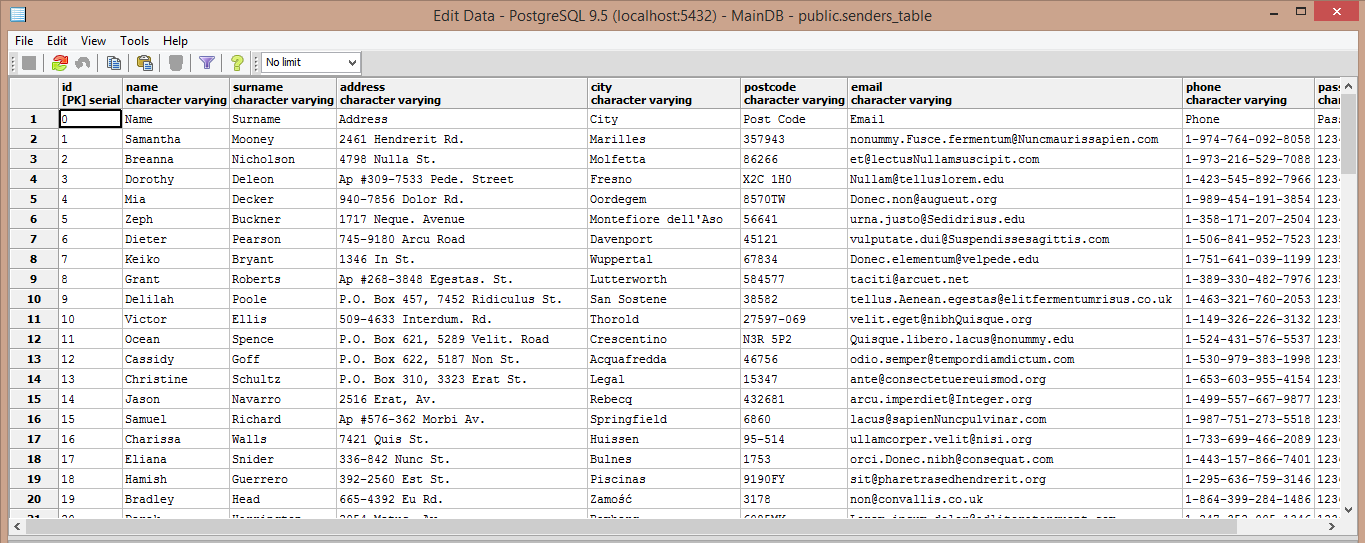
\includegraphics[width=4.5in]{pictures/screenshots/sendersscreen.png}
\caption{The senders table}
\label{SendersTable}
\end{figure}

\subsubsection*{Packing algorithm}
The implemented algorithm has the dimensions of the truck, and the extracts data from the package database and stores it in an array. It then computes the total dimensions of all the packages in the package array to check if they fit in one truck. If they fit in one truck the algorithm displays the message to the dispatcher and exits. Otherwise the algorithm, starts appending the items one by one onto the truck array. After appending each item, the algorithm checks whether the truck is full or not. If the truck is full a new truck is added and the item is appended onto the new truck.  And the algorithm is stuck in a lop that appends the items into the truck as long as there are trucks to append to or items to add. This was the first version of the implementation and it was going to be improved to get to level that was designed initial. Due to time constrains further implementation could not be done. Figure \ref{PackActivity} shows the UML activity diagram of the implemented algorithm. 

\begin{figure}[hbt!]
\centering
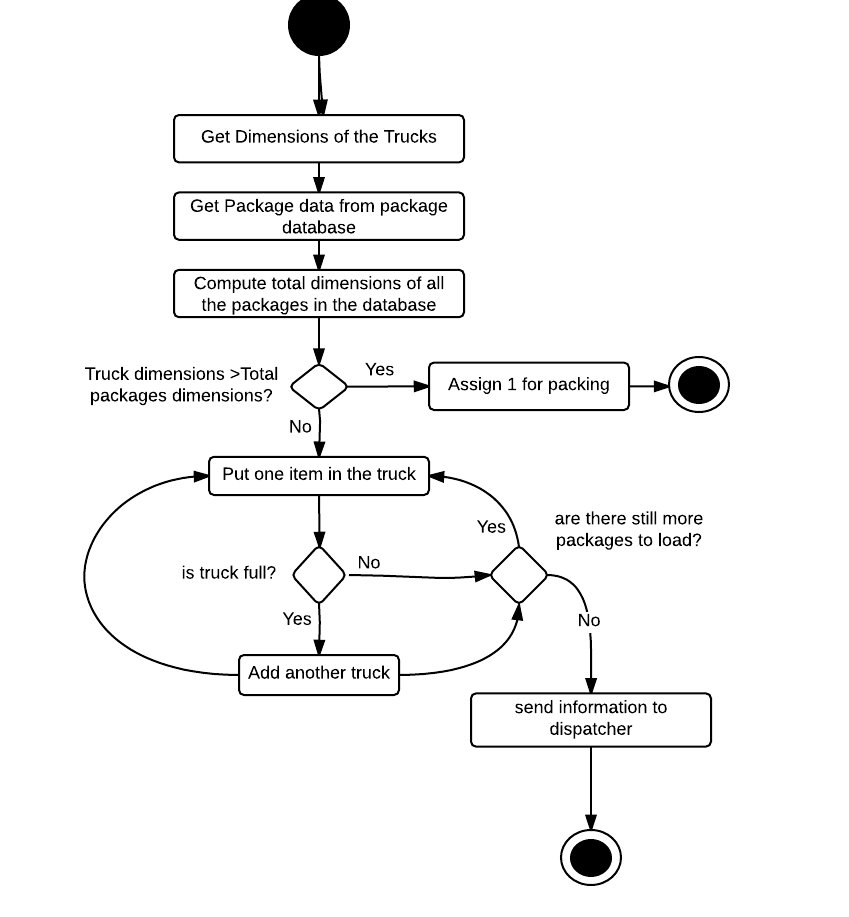
\includegraphics[width=4.5in]{pictures/ActivityDiagramPacking.png}
\caption{The packing algorithm activity diagram}
\label{PackActivity}
\end{figure}

Although the packing algorithm has not been linked to the front end. It has been implemented and extensively documented. One tool used for documenting it is doxygen. Figures \ref{}, \ref{} and \ref{} show the resulting in depth module description.

\begin{figure}[hbt!]
\centering
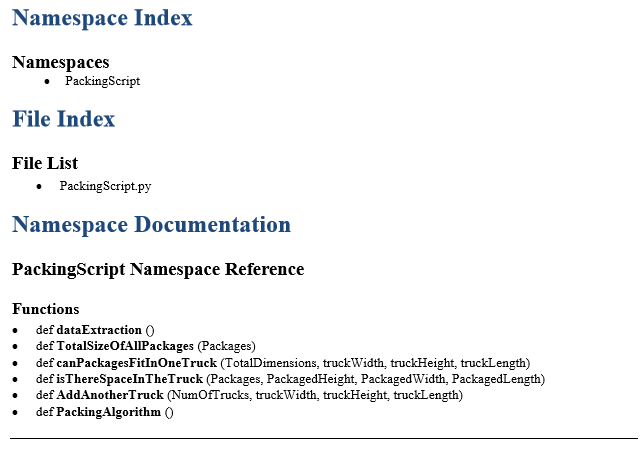
\includegraphics[width=4.5in]{pictures/doxygen/first_dox_pack.png}
\caption{Doxygen of the packing algorithm namespaces}
\label{DoxyOnePack}
\end{figure}

\begin{figure}[hbt!]
\centering
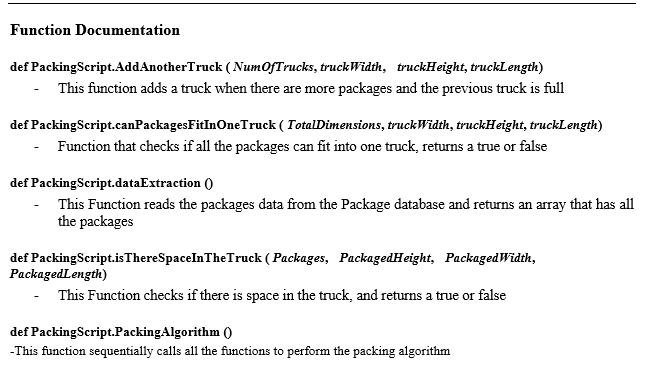
\includegraphics[width=4.5in]{pictures/doxygen/second_dox_pack.png}
\caption{Doxygen of the packing algorithm function documentation}
\label{DoxyTwoPack}
\end{figure}

\begin{figure}[hbt!]
\centering
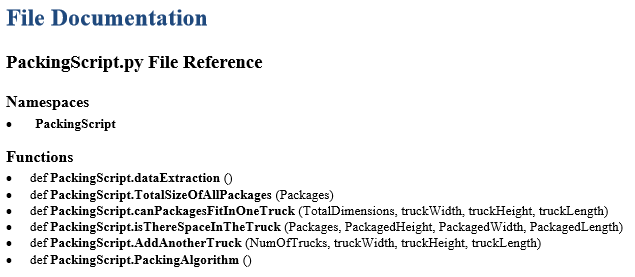
\includegraphics[width=4.5in]{pictures/doxygen/third_dox_pack.png}
\caption{Docxygen of the packing algorithm file documentation}
\label{DoxyThreePack}
\end{figure}


\section{Design Analysis}
The webpages for the system were successfully created. Databases to create dummy data to test the system was created, and a packing algorithm was written.In the early stages of the project extensive research was conducted and a design brief was document. Due to the time constraints the separately developed parts could not be concatenated to bring about an overall system. Even though the algorithms could not be joined to the rest of the software, basic functionality was achieved to demonstrate the basic functionality of the software.Extensive documentation of all modules that were planed are there for simplicity of future improvements of this project.

\newpage
\section{SCRUM}

The agile software development framework chosen for the project is the SCRUM method. This method is chosen because it is lightweight, simple to understand and easy to use. Scrum will be used to address complex problems, increase productivity and deliver a unique solution. An iterative process will be followed where one team is responsible for the front-end and the other team is responsible for the back-end. The process will be iterative whereby the front end team will develop the web pages and the back-end team will then link these pages to the server. It will also be assumed that product specifications will remain constant for the prototype phase with any changes being added after the development of the prototype.

\subsection{The project charter}
The various components of the project charter are described in the introduction of this document.
\subsection{Product Backlog}
The product backlog can be seen in Table \ref{ProductBacklogTable}.
\begin{table}[!hbt]
\centering
\caption{Product Backlog}
\label{ProductBacklogTable}
\begin{tabular}{|p{1cm}|p{8cm}|p{2cm}|p{1.2cm}|}
\hline
\textbf{ID} & \textbf{Story}                                                                                         & \textbf{Estimate} & \textbf{Priority} \\ \hline
1           & As a sender I need to be able to create an account                                                     & 10                & 1                 \\ \hline
2           & As a sender I need to be able to log in to my account                                                  & 2                 & 2                 \\ \hline
3           & As a sender I need to input the dimensions of my package                                               & 2                 & 3                 \\ \hline
4           & As a sender I want to input my details                                                                 & 3                 & 4                 \\ \hline
5           & As a sender I want to input the receiver's details                                                     & 2                 & 5                 \\ \hline
6           & As a sender I need to be able to pay for the services                                                  & 5                 & 6                 \\ \hline
7           & As a fleet assigment manager I need to be able run a route generation algorithm                        & 5                 & 7                 \\ \hline
8           & As a fleet assigment manager I need to see a list of packages in the depot                             & 1                 & 8                 \\ \hline
9           & As a driver I should be able to log in to my account                                                   & 1                 & 9                 \\ \hline
10          & As a driver I want to pick a vehicle and a route                                                       & 10                & 10                \\ \hline
11          & As a driver I need to see the contact details of my next delivery / pickup                             & 2                 & 11                \\ \hline
12          & As a driver I want to check off the packages I drop off / pickup                                       & 3                 & 12                \\ \hline
13          & As a sender I need to know when the parcel will be picked up                                           & 1                 & 13                \\ \hline
14          & As a sender I need to be able to know when the package will be delivered                               & 3                 & 14                \\ \hline
15          & As a receiver I need to receive a notification of the intended delivery                                & 1.5               & 15                \\ \hline
16          & As a receiver I need to check the estimated time of delivery                                           & 1                 & 16                \\ \hline
17          & As the CEO I want to see statistics on the clients                                                     & 4                 & 17                \\ \hline
18          & As the CEO I want to see statistics on the drivers                                                     & 4                 & 18                \\ \hline
19          & As the Vehicle Maintenance Manager I want to see vehicle statistics such as mileage                    & 6                 & 19                \\ \hline
20          & As the Vehicle Maintenance Manager I want to schedule the maintenance of vehicles                      & 5                 & 20                \\ \hline
21          & As the Accounts Officer I want to see the list of payments made (for bookeeping purposes)              & 6                 & 21                \\ \hline
22          & As the Accounts Officer I need to see a list of vehicle maintenance payments (for bookeeping purposes) & 5                 & 22                \\ \hline
23          & As the CEO I want to generate reports on income                                                        & 5                 & 23                \\ \hline
24          & As the CEO I want to generate reports on expenditure                                                   & 5                 & 24                \\ \hline
25          & As a driver I want to be able to request a day off                                                     & 6                 & 25                \\ \hline
26          & As a driver I should be able to log out of my account                                                  & 1                 & 26                \\ \hline
27          & As a sender I need to be able to log out of my account                                                 & 1                 & 27                \\ \hline
28          & As the Vehicle Maintenance Manager I want to see vehicle statistics such as fuel consumption           & 5                 & 28                \\ \hline
            &                                                                                                        & 105.5             &                   \\ \hline
\end{tabular}
\end{table}

\subsection{Sprint Backlog}

The sprint backlog can be seen in Table \ref{SprintBacklogTableFirst}, \ref{SprintBacklogTableSecond}, \ref{SprintBacklogTableThird} and \ref{SprintBacklogTableFourth}.



\begin{table}[!hbt]
\centering
\caption{Sprint backlog}
\label{SprintBacklogTableFirst}
\begin{tabular}{|p{1cm}|p{5cm}|p{5cm}|p{2cm}|}
\hline
\textbf{ID} & \textbf{Story}                                                                  & \textbf{Sprint backlog tasks}                                                                      & \textbf{Date} \\ \hline
1           & As a sender I need to be able to create an account                              & Create a django project                                                                            & 21/03/2016    \\ \hline
            &                                                                                 & Design database structure                                                                          & 21/03/2016    \\ \hline
            &                                                                                 & Create databases                                                                                   & 22/03/2016    \\ \hline
            &                                                                                 & Link page to the django server                                                                     & 22/03/2016    \\ \hline
            &                                                                                 & Save user account details in the database                                                          & 23/03/2016    \\ \hline
            &                                                                                 & Make a form where clients are able to create their accounts                                        & 23/03/2016    \\ \hline
2           & As a sender I need to be able to log in to my account                           & Make a log in page                                                                                 & 24/03/2016    \\ \hline
            &                                                                                 & Save log in details of senders in database                                                         & 24/03/2016    \\ \hline
3           & As a sender I need to input the dimensions of my package                        & The user is required to fill in the dimensions of their package. & 25/03/2016    \\ \hline
            &                                                                                 & Send the package dimensions to the packing algorithm                                               & 25/03/2016    \\ \hline
4           & As a sender I want to input my details                                          & Make a form where the sender can enter their details                                               & 26/03/2016    \\ \hline
            &                                                                                 & Store the sender's details in the database                                                         & 26/03/2016    \\ \hline
5           & As a sender I want to input the receiver's details                              & Make a form where the sender can enter the receiver's details                                      & 27/03/2016    \\ \hline
            &                                                                                 & Store the receiver's details in the database                                                       & 27/03/2016    \\ \hline
6           & As a sender I need to be able to pay for the services                           & Update the accounts and payments databases                                                         & 28/03/2016    \\ \hline
            &                                                                                 & Authorise the user's packages for transport                                                        & 28/03/2016    \\ \hline
            &                                                                                 & Create a payment page for the user                                                                 & 29/03/2016    \\ \hline
7           & As a fleet assigment manager I need to be able run a route generation algorithm & Have a button that allows the manager to run the route allocation algorithm                        & 29/03/2016    \\ \hline
8           & As a fleet assigment manager I need to see a list of packages in the depot      & Display a list of all the packages that are at the depot that need to be allocated routes          & 30/03/2016    \\ \hline
\end{tabular}
\end{table}

\begin{table}[!hbt]
\centering
\caption{Sprint backlog continued}
\label{SprintBacklogTableSecond}
\begin{tabular}{|p{1cm}|p{5cm}|p{5cm}|p{2cm}|}
\hline
\textbf{ID} & \textbf{Story}                                                             & \textbf{Sprint Backlog Tasks}                                                                    & \textbf{Date} \\ \hline
9           & As a driver I should be able to log in to my account                       & Make a driver list in the database                                                               & 31/03/2016    \\ \hline
            &                                                                            & Implement code to facilitate logging in by drivers                                               & 31/03/2016    \\ \hline
10          & As a driver I want to pick a vehicle and a route                           & Implement route assigning algorithm                                                              & 01/04/2016    \\ \hline
            &                                                                            & Implement packing algorithm                                                                      & 01/04/2016    \\ \hline
            &                                                                            & Implement a google map using the google maps API on the driver interface                         & 02/04/2016    \\ \hline
            &                                                                            & Implement a checklist of all items on  the driver's route on the driver interface                & 02/04/2016    \\ \hline
            &                                                                            & Display contact details of client on web page                                                    & 03/04/2016    \\ \hline
            &                                                                            & Implement a checklist option to choose between routes on the before page of the driver interface & 03/04/2016    \\ \hline
11          & As a driver I need to see the contact details of my next delivery / pickup & Display the contact details of current pickup/ delivery                                          & 04/04/2016    \\ \hline
12          & As a driver I want to check off the packages I drop off / pickup           & Implement a checklist for the packages on the driver's interface                                 & 04/04/2016    \\ \hline
13          & As a sender I need to know when the parcel will be picked up               & Implement code to calculate the estimated time of pickup                                         & 05/04/2016    \\ \hline
            &                                                                            & Display the value of the calculated time of pickup on the sender interface                       & 06/04/2016    \\ \hline
14          & As a sender I need to be able to know when the package will be delivered   & Calculate the ETA when the payment, and allocation of a package has been made                    & 06/04/2016    \\ \hline
            &                                                                            & Send the user a notification with the ETA                                                        & 07/04/2016    \\ \hline
            &                                                                            & Update the ETA on the user's interface                                                           & 08/04/2016    \\ \hline
15          & As a receiver I need to receive a notification of the intended delivery    & Implement code to send a notification when the ETD has been calculated                           & 09/04/2016    \\ \hline
\end{tabular}
\end{table}

\begin{table}[!hbt]
\centering
\caption{Sprint backlog continued}
\label{SprintBacklogTableThird}
\begin{tabular}{|p{1cm}|p{5cm}|p{5cm}|p{2cm}|}
\hline
\textbf{ID} & \textbf{Story}                                                                                         & \textbf{Sprint backlogs}                                                          & \textbf{Date} \\ \hline
16          & As a receiver I neeed to check the estimated time of delivery                                          & Display the ETD when it has been calculated                                       & 10/04/2016    \\ \hline
17          & As the CEO I want to see statistics on the clients                                                     & Calculate all the statistics on clients                                           & 11/04/2016    \\ \hline
            &                                                                                                        & Display the statistics on the CEO interface                                       & 11/04/2016    \\ \hline
18          & As the CEO I want to see statistics on the drivers                                                     & Calculate all the statistics on drivers                                           & 12/04/2016    \\ \hline
            &                                                                                                        & Display the statistics on the CEO interface                                       & 12/04/2016    \\ \hline
19          & As the Vehicle Maintenance Manager I want to see vehicle statistics such as mileage                    & Implement an algorithm that computes vehicle statistics                           & 13/04/2016    \\ \hline
            &                                                                                                        & Display the results of the algorithm                                              & 13/04/2016    \\ \hline
20          & As the Vehicle Maintenance Manager I want to schedule the maintenance of vehicles                      & Implement an algorithm that computes the need of a vehicle to undergo maintenance & 14/04/2016    \\ \hline
            &                                                                                                        & Add an undergo maintenance button                                                 & 14/04/2016    \\ \hline
            &                                                                                                        & Display the results of the algorithm                                              & 15/04/2016    \\ \hline
            &                                                                                                        & Update the list of available vehicles                                             & 15/04/2016    \\ \hline
21          & As the Accounts Officer I want to see the list of payments made (for bookeeping purposes)              & Fetch the payments information from the database                                  & 16/04/2016    \\ \hline
            &                                                                                                        & Display the payment information summary                                           & 16/04/2016    \\ \hline
22          & As the Accounts Officer I need to see a list of vehicle maintenance payments (for bookeeping purposes) & Fetch the payments information from the database                                  & 17/04/2016    \\ \hline
            &                                                                                                        & Display the payment information summary                                           & 17/04/2016    \\ \hline
23          & As the CEO I want to generate reports on income                                                        & Generate a pdf/report of the information the CEO is viewing                       & 18/04/2016    \\ \hline
            &                                                                                                        & Have a generate report button on the CEO's interface                              & 18/04/2016    \\ \hline
\end{tabular}
\end{table}

\begin{table}[!hbt]
\centering
\caption{Sprint backlog continued}
\label{SprintBacklogTableFourth}
\begin{tabular}{|p{1cm}|p{5cm}|p{5cm}|p{2cm}|}
\hline
\textbf{ID} & \textbf{Story}                                                                               & \textbf{Sprint backlogs}                                                      & \textbf{Date} \\ \hline
24          & As the CEO I want to generate reports on expenditure                                         & Generate a pdf/report of the information the CEO is viewing                   & 19/04/2016    \\ \hline
            &                                                                                              & Have a generate report button on the CEO's interface                          & 19/04/2016    \\ \hline
25          & As a driver I want to be able to request a day off                                           & Have a request day off button on the page before page of the driver interface & 20/04/2016    \\ \hline
            &                                                                                              & Implement code to take the driver off the available drivers list              & 22/04/2016    \\ \hline
26          & As a driver I should be able to log out of my account                                        & Implement code to facilitate logging out by drivers                           & 23/04/2016    \\ \hline
27          & As a sender I need to be able to log out of my account                                       & Make a log out button on the web page                                         & 24/04/2016    \\ \hline
            &                                                                                              & Revoke the user's access                                                      & 24/04/2016    \\ \hline
28          & As the Vehicle Maintenance Manager I want to see vehicle statistics such as fuel consumption &                                                                               & 26/04/2016    \\ \hline
\end{tabular}
\end{table}

\subsection{Sprint retrospective}

The project consisted of 3 sprints which lasted 1 week each. This consisted of two daily meetings that happened on a Monday and Friday of each sprint. \\

Sprint 1: 21 March \textemdash  27 March\\\\
This sprint goal was to achieve the first 5 (Element 1-5) tasks on the sprint backlog.  These tasks were completed in time with a few adjustments. In element 1, forms for clients to create their accounts was removed and added as a server task instead. The user accounts are manually stored on the database for the prototype stage. The account creation page will now be done once CourierJZ approves the prototype design as this page may lead to developer complications.  In element 4, no form for the pickup location was added since it will be stored in the user's profile and thus simplify the act of sending a package.\\

Sprint 2: 28 March \textemdash 3 April\\\\
This sprint goal was to achieve elements 6\textemdash10 on the sprint backlog. Only tasks 7\textemdash9 were completed. This was due to the complexity of element 10 and the programmers time being limited by other commitments. For element 6 the payment management system was not implemented due to it not being an integral part of the prototype system. The information about the user's payment details (i.e. Credit card details) will now be stored in the users profile when implemented, this will make the process of sending a package simpler as the card details will not need to be entered each time as in is saved on the database.\\

Sprint 3: 4 April \textemdash 10 April\\\\
This was the last sprint for the prototype stage. For this cycle elements 10\textemdash16 needed to be completed for the last sprint. From element 10, the route assignment algorithm was not implemented. This is because the developers decided to focus on one algorithm (packing algorithm) due to time constraints. During the prototype stage, for simplicity the developers decided to only implement one driver profile, so there was only one route determined, therefore the page for drivers to pick routes was not necessary. For element 12, the check list was replaced by a submit button for each user. This was done so that when items were ticked, they could not mistakenly be unticked in the delivery process. Element 13 and 14 were removed from the list because the shortest distance algorithm was not implemented, so delivery times could not be correctly assigned for each package. Element 15 and 16 were combined into a receiver page with the relevant details being accessible by inputting the tracking ID into the receiver dashboard.\\

\begin{figure}[hbt!]
\centering
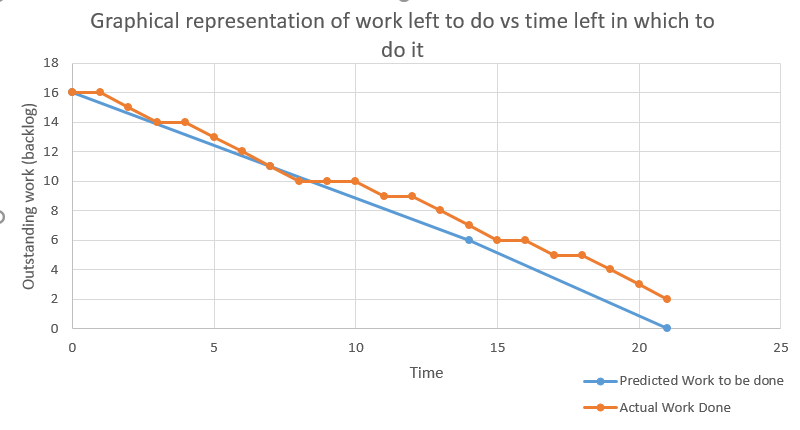
\includegraphics[width=5in]{pictures/chart.png}
\caption{Burn down chart of prototype}
\label{BurndownChart}
\end{figure}

It can be seen from Figure \ref{BurndownChart} that in the beginning of the developmental process of the prototype,the project was on track. However towards the end, the actual work that was being performed was not meeting the targets. This could be because the work that needed to be performed was underestimated and therefore time was not allocated correctly. Care must be taken to ensure that these task are completed in the nearby future, otherwise the project has a high risk of not being completed in time. 

\section{Conclusion}
A solution to the problem was developed. This solution involved devising algorithms based on adapting the existing solutions to the needs of CourierJZ. A web based application was developed, it interacts with all the stake holders and it was insures that as much information as possible is relayed to all stake holders to minimize and inconvenience and maximize profits and efficiency for CourierJZ. Although the implementation was incomplete the documentation explains clearly the intend path of design

\begin{appendix}
  \listoffigures
  \listoftables
\end{appendix}

\begin{thebibliography}{sorting}

\bibitem{DHL} 
Unknown. www.dhl.co.za. Last accessed 08 April 2016.
\bibitem{Aramex} 
Unknown. www.aramex.co.za. Last accessed 08 April 2016.
\bibitem{Fastway} 
Unknown. "Fastway Couriers". www.fastway.co.za. Last accessed 08 April 2016.
\bibitem{Telogis}
Unknown. "Telogis Distributions". http://www.telogis.com/industries/distribution. Last accessed 09 April 2016.
\bibitem{IDSystems}
"Vehicle Management Systems (VMS) :  Constant Connection, constant improvement". http://www.id-systems.com/about-vms/. Last accessed 09 April 2016.
\bibitem{Ichoua}
Ichoua S, Gendreau M, and Potvin J. "Diversion Issues in Real-Time Vehicle Dispatching". Transportation Science, © 2000 INFORMS 0041-1655/00/3404-0426  Vol. 34, No. 4, November 2000.
\bibitem{Abbaspour}
Abbaspour R. A and Samadzadegan F. "An Evolutionary Solution for Multimodal Shortest Path Problem in Metropolises", UDC 519.8, DOI:10.2298/CSIS090710024A. 
\bibitem{Delling}
Delling D and Wagner D. "Time-Dependent Route Planning. Robust and Online Large-Scale Optimization". Volume 5868 of the series Lecture Notes in Computer Science, pp 207-230.
\bibitem{Psraftis}
Psraftis H. N. "Dynamic Vehicle Routing - Status and Prospects". Annals of Operations Research 61(1995)143-164. Pp 143 - 164.
\bibitem{Madsen}
Madsen B. G. O, Allan Larsen A, Solomon M. M. "Dynamic Vehicle Routing Systems – Survey and Classification".
\bibitem{Hong}
Hong C. K, Benkrid  X., Iturbe A., Erdogan T, and Arslan T. “An FPGA task allocator with preliminary First-Fit 2D packing algorithms” ,Adaptive Hardware and Systems (AHS), 2011 NASA/ESA Conference on IEEE Conference Publications.
\bibitem{Zhu}
Zhu Z., Sui J. and Yang L., "Bin-packing Algorithms for Periodic Task Scheduling “ Information Engineering (ICIE), 2010 WASE International Conference on , 2010, Volume: 2, Pages: 207 - 210, DOI: 10.1109/ICIE.2010.145, IEEE Conference Publications.
\bibitem{Huang}
Huang L., Liu Z., and Liu Z., “An improved lowest-level best-fit algorithm with memory for the 2D rectangular packing problem”, Information Science, Electronics and Electrical Engineering (ISEEE), 2014 International Conference on ,2014, Volume: 2 ,Pages: 1279 - 1282, DOI: 10.1109/InfoSEEE.2014.6947877, IEEE Conference Publications.




\end{thebibliography}



















%----------------------------------------------------------------------------------------



\end{document}